\documentclass[12pt,a4paper]{article}

\usepackage[utf8]{inputenc}
\usepackage[margin=1in]{geometry}
\usepackage{amsthm,amsfonts}
\usepackage{mathrsfs}
\usepackage{amsmath,amssymb}
\usepackage{mathtools}
\usepackage[hidelinks,
            colorlinks=true,
            linkcolor=blue,
            citecolor=blue,
            urlcolor=blue]{hyperref}
\usepackage{tikz-cd}
\usepackage{kbordermatrix}
\usepackage{enumitem}
\usepackage{xcolor}
\usepackage{graphicx}
\usepackage{caption}
\usepackage{subcaption}
\usepackage{url}
\usepackage[capitalise,nameinlink,noabbrev]{cleveref}



% Miscellaneous
\newcommand{\abs}[1]{\lvert {#1} \rvert}
% https://tex.stackexchange.com/a/5825
\def\multiset#1#2{\ensuremath{\left(\kern-.3em\left(\genfrac{}{}{0pt}{}{#1}{#2}\right)\kern-.3em\right)}}

% Common mathbb
\renewcommand{\AA}{\mathbb{A}}
\newcommand{\KK}{\mathbb{K}}
\newcommand{\NN}{\mathbb{N}}
\newcommand{\PP}{\mathbb{P}}
\newcommand{\CC}{\mathbb{C}}
\newcommand{\RR}{\mathbb{R}}
\newcommand{\QQ}{\mathbb{Q}}
\newcommand{\ZZ}{\mathbb{Z}}

% Common commutative algebra
\DeclareMathOperator{\Ann}{Ann}
\DeclareMathOperator{\Betti}{Betti}
\DeclareMathOperator{\Ext}{Ext}
\DeclareMathOperator{\HF}{HF}
\DeclareMathOperator{\HP}{HP}
\DeclareMathOperator{\HS}{HS}
\DeclareMathOperator{\Hom}{Hom}
\DeclareMathOperator{\image}{im}
\DeclareMathOperator{\init}{in}
\DeclareMathOperator{\pdim}{pdim}
\DeclareMathOperator{\reg}{reg}
\DeclareMathOperator{\Tor}{Tor}

% Common combinatorics
\DeclareMathOperator{\sstar}{\text{st}}
\DeclareMathOperator{\link}{\text{lk}}
% \newcommand{\GMA}[1]{\mathsf{B}_{#1}}
% \renewcommand{\L}{\mathcal{L}}
% \DeclareMathOperator{\rk}{rk}

% Some environments
\newtheorem{theorem}{Theorem}[section]
\newtheorem{lemma}[theorem]{Lemma}
\newtheorem{corollary}[theorem]{Corollary}
\newtheorem{proposition}[theorem]{Proposition}
\newtheorem{conjecture}[theorem]{Conjecture}
\newtheorem{question}[theorem]{Question}
\newtheorem*{tldr}{TL;DR}


\theoremstyle{definition}
\newtheorem{definition}[theorem]{Definition}
\AtEndEnvironment{definition}{\null\hfill\ensuremath{\bullet}}
\newtheorem{remark}[theorem]{Remark}
\newtheorem{example}[theorem]{Example}
\AtEndEnvironment{example}{\null\hfill\ensuremath{\blacksquare}}
\newtheorem{exercise}[theorem]{Exercise}
\AtEndEnvironment{exercise}{\null\hfill\ensuremath{\blacktriangledown}}

\numberwithin{equation}{section}

% cf https://tex.stackexchange.com/a/732053/5001
\AddToHook{env/lemma/begin}{\crefalias{theorem}{lemma}}
\AddToHook{env/corollary/begin}{\crefalias{theorem}{corollary}}
\AddToHook{env/proposition/begin}{\crefalias{theorem}{proposition}}
\AddToHook{env/conjecture/begin}{\crefalias{theorem}{conjecture}}
\AddToHook{env/question/begin}{\crefalias{theorem}{question}}
\AddToHook{env/definition/begin}{\crefalias{theorem}{definition}}
\AddToHook{env/remark/begin}{\crefalias{theorem}{remark}}
\AddToHook{env/example/begin}{\crefalias{theorem}{example}}
\AddToHook{env/exercise/begin}{\crefalias{theorem}{exercise}}

% \crefname{lemma}{lemma}{lemmas}
% \crefname{corollary}{corollary}{corollaries}
% \crefname{proposition}{proposition}{propositions}
% \crefname{conjecture}{conjecture}{conjectures}
% \crefname{question}{question}{questions}
% \crefname{definition}{definition}{definitions}
% \crefname{remark}{remark}{remarks}
% \crefname{example}{example}{examples}
% \crefname{exercise}{exercise}{exercises}

% \Crefname{lemma}{Lemma}{Lemmas}
% \Crefname{corollary}{Corollary}{Corollaries}
% \Crefname{proposition}{Proposition}{Propositions}
% \Crefname{conjecture}{Conjecture}{Conjectures}
% \Crefname{question}{Question}{Questions}
% \Crefname{definition}{Definition}{Definitions}
% \Crefname{remark}{Remark}{Remarks}
% \Crefname{example}{Example}{Examples}
% \Crefname{exercise}{Exercise}{Exercises}




\title{ISMaRT Project Preliminaries}

\begin{document}
\author{}
\date{}

\maketitle

\tableofcontents

\newpage
\section{Crash Course in Ring Theory}
\noindent\textit{Rings encode relations.}

\vspace*{2.5cm}

\noindent Often in applications, one wishes to understand the solutions to a system of equations.
When these equations are polynomials, tools in commutative algebra and algebraic geometry have been developed to describe these solution sets.
When the system of polynomial equations consists of homogeneous polynomials, the solution sets lie in projective space. 
Because projective space is covered by affine patches (places where polynomials need not be homogeneous), much work has been put into understanding objects in the projective setting.

\vspace*{2.5cm}

\begin{tldr}
    \phantom{ }
    \begin{itemize}
        \item Quotienting a ring by an ideal is setting \emph{relations} on elements of the ring.

        \item Modules are basically vector spaces over a ring (as opposed to a field).

        \item Artinian rings are finite-dimensional vector spaces which can be stratified via a \emph{grading}.
    \end{itemize}
\end{tldr}

\vspace*{2.5cm}

\newpage

\subsection{Fundamentals}
In my opinion, many of the rings you encounter in undergraduate algebra are very boring or their interesting properties aren't motivated nor explored enough.
To me, rings act as a proxy to be able to encode relations about whatever object you are studying.
This manifests by, for instance, taking a polynomial ring and quotienting it by an ideal where the generators of the ideal describe the \emph{relations} you want to impose, i.e., information you want to discard.

\begin{example}
    Consider the polynomial ring $\KK[x,y,z]$, and let $I = (x^2 - yz)$.
    By forming the quotient ring $R/I$, we are basically imposing the relation that $x^2 - yz = 0$, or alternatively, $x^2 = yz$.
    So when working with elements in $R/I$, we can replace any instances of $x^2$ with $yz$, or vice versa.
\end{example}

A fundamental insight is that ideals in polynomial rings correspond (in a precise sense) with geometric objects in affine or projective space.
So, to understand the geoemtric object---something you typically want to know more information about---you can try to understand its corresponding algebra.
This connection is explored more in the next section.

\begin{definition}
    Let $R = \KK[x_1,\dots,x_n]$.
    A polynomial $f \in R$ is \emph{homogeneous} if all of the monomials in $f$ have the same degree.
    An ideal $I \subseteq R$ is \emph{homogeneous} if it can be generated by homogeneous elements, i.e., $I = (f_1,\dots,f_r)$ where each $f_i$ is homogeneous.
\end{definition}

\begin{example}
    Let $R = \KK[x,y,z]$.
    The polynomial $x^2 + xy$ is homogeneous, but the polynomial $x^2 + x$ is not.
    The ideal
    \begin{equation*}
        I = (2x^3 - 2z^3 + x^2 + y^2 + z^2, x^3 - y^3 - z^3, y^3 + x^2 + y^2 + z^2)
    \end{equation*}
    might not look homogeneous, but this is a byproduct of how we wrote the generators.
    We can show that
    \begin{equation*}
        I = (x^2 + y^2 + z^2, x^3 - z^3, y^3),
    \end{equation*}
    and so, by definition of $I$, every element of $I$ is generated by homogeneous elements; i.e., $I$ \emph{is} a homogeneous ideal.
\end{example}

I'm going to skip over a lot of content, but the short story is that we \emph{really} like homogeneous ideals for a couple of reasons:
\begin{itemize}
    \item When $I$ is homogeneous, the quotient ring $R/I$ comes equipped with \emph{gradings}, so we can do computations with them.

    \item Homogeneous ideals describe geometric objects in projective space (here, geometry works out a lot nicer than classical geometry).
\end{itemize}

\vspace*{1cm}

\noindent {\bf See Also}: Appendix A.2 of~\cite{schenck_computational_2003}.

\vspace*{1cm}


\subsection{Geometric intuition}
Throughout, let $R = \KK[x_1,\dots,x_n]$---the polynomial ring in $n$ variables over the field $\KK$.
Furthermore, let $I \subseteq R$ be an ideal of $R$ so that we can consider the quotient $M = R/I$.

For all intents and purposes, you can think of \emph{affine space}, denoted $\AA_{\KK}^n$, as the points $(a_1,\dots,a_n)$.
When we draw pictures in calculus we are usually drawing points in $\RR^n = \AA_{\RR}^n$.
However, for geometry to really shine, we need to work projectively.
So, \emph{projective space}, denoted $\PP_{\KK}^n$, consists of the points $[a_0 \colon \dots \colon a_n]$ modulo the relation that two points which are non-zero multiples of each other define the same point, and there is no point $[0 \colon \dots \colon 0]$.
Intuitively, think of $\PP^n$ as $\AA^{n+1}$ where we have thrown out the origin and then identified points up to scaling.

\begin{definition}
    The \emph{variety} defined by a homogeneous ideal $I$ is the set of points
    \begin{equation*}
        \mathbf{V}(I) = \{ [a_0 \colon \dots \colon a_n] \in \PP^n \colon f(a_0 \colon \dots \colon a_n) = 0 \text{ for all } f \in I \}.
    \end{equation*}
    Similarly, the \emph{ideal} defined by a variety $V \subseteq \PP^n$ is the set of elements
    \begin{equation*}
        \mathbf{I}(V) = \{ f \in R \colon f(x) = 0 \text{ for all } x \in V \}.
    \end{equation*}
    For a variety $V \subseteq \PP^n$, its \emph{coordinate ring} is the quotient $\KK[V] \coloneqq R/I$;
    polynomials which vanish everywhere on $V$ are $0$ in $\KK[V]$.
\end{definition}

\begin{example}
    In the affine plane, the variety $\mathbf{V}(y - x^2)$ is a parabola as it consists of the points satisfying $y - x^2 = 0$.
\end{example}

\begin{example}
    The \emph{twisted cubic} is the curve $C$ in $\PP^3$ defined by the equations $xz - y^2$, $yw - z^2$, and $xw - yz$; i.e.,
    \begin{equation*}
        C = \mathbf{V}(xz - y^2, yw - z^2, xw -yz).
    \end{equation*}
    Alternatively, $C$ is parametrically described by the image of $\nu \colon [s \colon t] \mapsto [s^3 \colon s^2 t \colon s t^2 \colon t^3]$.
    You should verify that the parametric description of $C$ via $[s^3 \colon s^2 t \colon s t^2 \colon t^3]$ satisfies the defining equations of $C$.
    (Hint: Think of setting each coordinate as a variable---i.e., $s^3 \mapsto x, s^2 t \mapsto y, \dots$---and make the appropriate substitutions into the defining equations to ensure you get $0$ for each one.)

    Since there are four coordinates, we can't effectively visualize the entire curve, but by projecting via setting $s=1$, we can view a part of the curve as the points $(t, t^2, t^3)$ (you can plot this!).
    See \href{https://en.wikipedia.org/wiki/Twisted_cubic}{Wikipedia} for a visualization or more explicit details.
\end{example}


What's the point?
By passing back and forth between a variety and its defining ideal (or an ideal and its variety), understanding one side of the correspondence helps to understand the other side, too.
For instance, there is a close connection to computing chains of prime ideals in $I$ to the dimension of $\mathbf{V}(I)$.

Furthermore, computationally working with $\mathbf{V}(I)$ can be quite difficult.
Sure, you might be able to find defining equations of the variety, but how do you actually get a concrete point (or all points) on a variety?
In arithmetic geometry (think: number theory), this amount to understanding the \emph{rational points} on a variety, a notoriously hard problem resulting in many conjectures (e.g, \href{https://en.wikipedia.org/wiki/Mordell%E2%80%93Weil_theorem}{Mordell Weil theorem} or one of the Millenium Prize Problems, the \href{https://en.wikipedia.org/wiki/Birch_and_Swinnerton-Dyer_conjecture}{Birch and Swinnerton-Dyer conjecture}).

On the other hand, it turns out \emph{polynomials} work very well on computers.
In general, solving systems of polynomial equations is also very hard.
Think back to Lagrange multipliers from Calculus III: there was not a consistent, tried-and-true method to solving those systems of polynomials.
However, with the help of Gr\"obner bases and Buchberger's Algorithm, we can perform some sort of pseudo-Gaussian elimination on the system of polynomials to solve it.

\begin{remark}
    While this approach works, it is also typically pretty expensive.
    Solving a system of $n$ linear equations (i.e., Guassian elimination) is $O(n^3)$, whereas solving a system of polynomial equations in $n$ variables---each of degree at most $d$---is $O(d^{2^n})$.
\end{remark}

\vspace*{1cm}

\noindent {\bf See Also}: Section 2.1 of \cite{schenck_computational_2003}.

\vspace*{1cm}


\subsection{Dimension theory}
A common strategy to understand a mathematical object is to assign invariants to it, and then to determine how well that invariant ``classifies'' the object.
To be an invariant typically means that if $A \cong B$, then $\text{invariant}(A) = \text{invariant}(B)$.
Another way to phrase this is via the contrapositive: if $\text{invariant}(A) \neq \text{invariant}(B)$, then $A \not\cong B$.
Moreover, the converse to the invariant definition is generally not true either; invariants are a \emph{coarser} description of an object.
For example, two matrices can have the same eigenvalues, but just because they have the same eigenvalues does not imply that they are the same matrices.

A quintessential invariant type is \emph{dimension} (however it is defined for a class of objects).
For instance, when a field $\KK$ is fixed, finite-dimensional $\KK$-vector spaces are completely determined by their dimension; that is, if $V$ and $W$ are finite-dimensional $\KK$-vector spaces, then $V \cong W$ if and only if $\dim_{\KK}{V} = \dim_{\KK}{W}$.
Trying to abstract this approach, the \emph{Hilbert function} and \emph{Hilbert series} are an invariant of a module that measures the ``growth'' of the graded components of the module as the grading ``grows''.

\begin{definition}[Kind of]
    Let $R$ be a ring.
    An \emph{$R$-module} is an ``$R$-vector space''.
\end{definition}

While it might seem that vector spaces can be quite complicated, they are actually some of the simplest and nicest objects you can have.
They allow you to do ``nice'' linear algebra computations, are ``finite'', and are determined by their dimension (and field).
In commutative algebra, modules take their place: the scalars now come from a (commutative) ring, versus simply a field.

This substitution of ``ring'' for ``field'' is a little simplistic, but it absolutely wrecks many of the conveniences of vector spaces.
Remember: the goal in mathematics is to turn your problem into a linear algebra problem so that you can compute it; this requires working over a field.
For modules, they are typically \emph{infinite-dimensional} as $\KK$-vector spaces (so long, computations!).

In our setting with polynomial rings, our modules come with ``gradings'' where ``degree'' acts as a stratification for the module, allowing us to think about this infinite-dimensional objects as being decomposed into finite-dimensional graded components.
For example, consider the polynomial ring in two variable $\KK[x,y]$.
When viewed as a $\KK$-vector space, even though it is infinite-dimensional, you can write down a basis for it; e.g., $\{ 1, x, x^2, x^3, \dots \}$.
Moreover, you could choose to organize these basis elements by their usual \emph{degree}:
\begin{center}
    {\renewcommand{\arraystretch}{2.5}
    \begin{tabular}{|c||c|c|c|c|c|}
        \hline
        Degree & 0 & 1 & 2 & 3 & \dots \\
        \hline
        Basis & 1 & $x, y$ & $x^2, xy, y^2$ & $x^3, x^2 y, x y^2, y^3$ & \dots \\
        \hline
    \end{tabular}}
\end{center}
This allows us to think of a module (with a grading) as being decomposed like
\begin{equation*}
    M = \bigoplus_d M_d,
\end{equation*}
where each $M_d$ is a finite-dimensional $\KK$-vector space.
This might seem like overkill, but it will prove to be very useful.

\begin{definition}
    Let $R = \KK[x_1,\dots,x_n]$ and let $M$ be an $R$-module.
    The \emph{Hilbert function} of $M$ is the integer-valued function $\HF_M \colon \ZZ \to \NN$ where $\HF_M(d) = \dim_{\KK}(M_d)$.
    The Hilbert function can be collected into a generating series, called the \emph{Hilbert series} of $M$:
    \begin{equation*}
        \HS(M) = \sum_{k=0}^\infty \HF_M(k) t^k.
    \end{equation*}
    Note that since we are considering $\HS(M)$ as a \emph{generating} series, this just means that 
    \begin{itemize}
        \item it is a power series (we don't care about where it converges), and
        \item the coefficients record or count something---in this case, the Hilbert function or dimension of $M_d$ as a $\KK$-vector space.
    \end{itemize}
\end{definition}

\begin{exercise}\label{exercise: hilbert polynomial ring}
    Try to compute the Hilbert series for $\KK[x_1]$, $\KK[x_1,x_2]$, and $\KK[x_1,x_2,x_3]$.
    Now, compute the Hilbert series for $\KK[x_1,\dots,x_n]$.
    (Hint: The ``stars-and-bars'' counting argument might prove useful.
    Alternatively, think about how to \emph{choose} degree $1$ monomials in order to construct a monomial of degree $d$.)
\end{exercise}

\begin{exercise}
    When $R = \KK[x_1,\dots,x_n]$, the Hilbert series can be expressed as a rational function $P(t) / Q(t)$.
    Take the Hilbert series from the previous exercise and express them as rational functions.
    For example, if $R = \KK[x_1]$ and $M = R$, then
    \begin{equation*}
        \HS(M) = \sum_{k=0}^\infty \HF_M(k) t^k = \sum_{k=0}^\infty t^k = \frac{1}{1-t}.
    \end{equation*}
\end{exercise}

\begin{proposition}
    When $R = \KK[x_1,\dots,x_n]$ and $M$ is an $R$-module, the Hilbert function is eventually a polynomial; i.e., for $k \gg 0$, $\HF_M(k) = P(k)$ for some polynomial $P$.
    This polynomial is called the \emph{Hilbert polynomial} of $M$.
\end{proposition}

What this means is that while the Hilbert function can do wild things at the start, the asymptotic behavior is eventually polynomial.
Suppose $M = R/I = \KK[V]$, so that $M$ is the coordinate ring of a variety $V$.
Remarkably, the Hilbert polynomial contains information about \emph{geoemtric} invariants of $V$: things like the degree, genus, and dimension of $V$.
In general, computing the Hilbert polynomial is quite hard, so a good first step is determining the Hilbert function/series.

Our old, trusty pal \emph{induction} is often times a good way to go about computing these kinds of things.
Usually, this approach entails an induction on the dimension, number of variables, etc.
In commutative algebra, one way of ``dropping dimension'' is to find a \emph{non-zero-divisor} in your ring.

\begin{definition}
    In a commutative ring $R$, an element $f$ is called a \emph{zero-divisor} if there exists some $r \in R$ such that $r \cdot f = 0$.
    Given $f \in R$, if there is no such $r$, then $f$ is called a \emph{non-zero-divisor} (here, ``non'' is modifying ``zero-divisor'', i.e., we mean $f$ is \emph{not} a zero-divisor).
\end{definition}

A lot of rings you encounter in undergraduate algebra are \emph{(integral) domains}, which by definition, have no zero-divisors.
However, in our setting--and most commutative algebra settings---we start with a domain (think: polynomial ring) and then introduce relations (think: ideal).
These relations yield lots of zero-divisors: if $f \in I$, then $r \cdot f \in I$ for all $r \in R$, and so $rf = 0$ in $R/I$.
However, if we can find a \emph{non}-zero-divisor $g$ in $R/I$, then we can basically ``chop down'' $R/I$ with $g$ to get a ``smaller'' ring without much loss of information.

\begin{example}
    Just as we can regard $\KK$ as a $\KK$-vector space, we can regard $R$ as an $R$-module.
    Let $R(i)$ denote $R$ (as an $R$-module) where we think of the generator as being in degree $-i$; this means that $R(-i)_d = R_{d-i}$.
    For example, $\KK[x,y](-2)$ will look like
    \begin{center}
    {\renewcommand{\arraystretch}{1.5}
    \begin{tabular}{|c|c|c|c|c|c|}
        \hline
        Degree $i$ & 0 & 1 & 2 & 3 & $\dots$ \\
        \hline
        Basis of ${\KK[x,y]}_i$ & $1$ & $x, y$ & $x^2, xy, y^2$ & $\dots$ & $\dots$ \\
        \hline
        Basis of ${\KK[x,y](-2)}_i$ & $0$ & $0$ & $1$ & $x, y$ & $\dots$ \\
        \hline
    \end{tabular}}
    \end{center}

    Why should this bookkeeping matter?
    Suppose $R$ is the polynomial ring $\KK[x_1,\dots,x_n]$ regarded as an $R$-module over itself, and let $f \in R_i$.
    We then have the map
    \begin{equation*}
        \cdot f \colon R \longrightarrow R \quad \text{where} \quad g \mapsto f \cdot g;
    \end{equation*}
    so, $\cdot f$ is the map from $R$ to itself given by multiplication by $f$.
    This is a very natural map encountered in the wild (in a rough sense, when $f$ is a non-zero-divisor, it corresponds to slicing $V(R)$ with $V(f)$), but importantly, it is \emph{not} a map of graded modules: it sends $1$ (something of degree $0$) to $f$ (something of degree $i$).
    The hack is to just shift the grading so that degree $0$ objects line up; that is, declare $1$ to have degree $i$ in the source module, we \emph{do} have a graded map
    \begin{equation*}
        R(-i) \xlongrightarrow[]{\cdot f} R.
    \end{equation*}
\end{example}

\vspace*{1cm}

\noindent {\bf See Also}: Section 2.2 of \cite{schenck_computational_2003}.

\vspace*{1cm}


\subsection{Artinian algebras}
\begin{definition}
    Let $R = \KK[x_1,\dots,x_n]$ and $I \subseteq R$ be a homogeneous ideal, and set $A \coloneqq R/I$.
    We say $A$ is Artinian if any of the following equivalent conditions hold:
    \begin{itemize}
        \item $\HF_A(i) = 0$ for $i \gg 0$.
        \item $A_i = 0$ for $i \gg 0$.
        \item $\HS(A)$ is a polynomial.
        \item $\dim_\KK(A) < \infty$.
        \item The \emph{Krull dimension} of $A$ is $0$.
    \end{itemize}
\end{definition}

\begin{example}
    \label{example:artinian-algebra}
    Let $R = \KK[x,y,z]$, $I = (x^2, y^2, z^2)$, and set $A = R/I$.
    We can list out the generators of $R$ and $A$ in each degree:
    
    \begin{center}
    {\renewcommand{\arraystretch}{2.5}
    \begin{tabular}{|c||c|c|c|c|c|c|}
        \hline
        $d$ & $0$ & $1$ & $2$ & $3$ & $4$ \\
        \hline
        \hline
        gens($R_d$) & $1$ & $\substack{x \\ y \\ z}$ & $\substack{x^2 \\ y^2 \\ z^2} \quad \substack{xy \\ xz \\ yz}$ & $\substack{x^3 \\ y^3 \\ z^3} \quad \substack{x^2 y \\ x^2 z} \quad \substack{y^2 x \\ y^2 z} \quad \substack{x z^2 \\ y z^2} \quad \substack{xyz}$ & $\dots$ \\
        \hline
        $\dim_\KK(R_d)$ & $1$ & $3$ & $6$ & $10$ & $15$ \\
        \hline
        \hline
        gens($A_d$) & $1$ & $\substack{x \\ y \\ z}$ & $\substack{xy \\ xz \\ yz}$ & $xyz$ & $\emptyset$ \\
        \hline
        $\dim_\KK(A_d)$ & $1$ & $3$ & $3$ & $1$ & $0$ \\
        \hline
    \end{tabular}
    }
    \end{center}
\end{example}

\begin{exercise}
    Construct a similar table as in \Cref{example:artinian-algebra}, but for $R = \KK[x,y,z]$ and $I = (x^2, y^2, z^3)$.
    Why is $A = R/I$ Artinian?
\end{exercise}


\subsection{Macaulay2 Code}
\begin{verbatim}
-- Example 1.3 (homogeneous ideals)
R = QQ[x,y,z]
I = ideal(2*x^3 - 2*z^3 + x^2 + y^2 + z^2, x^3 - y^3 - z^3, y^3 + x^2 + y^2 + z^2)
J = ideal(x^2 + y^2 + z^2, x^3 - z^3, y^3)
I == J

--  Example 1.6 (twisted cubic)
restart
R = QQ[x,y,z,w]
S = QQ[s,t]
nu = map(S, R, {s^3, s^2 * t, s * t^2, t^3})
I = kernel nu


-- Exercise 1.10 (Hilbert series for KK[x_1,...,x_n])
restart
n = 3
R = QQ[x_1..x_n]
apply(0..10, i -> hilbertFunction(i, R))


-- Exercise 1.11 (Hilbert series for KK[x_1,...,x_n] as P(t)/Q(t))
hilbertSeries R


-- Example 1.14 (Bases for KK[x,y] and KK[x,y](-2))
netList apply(5, i -> flatten entries basis(i, R))
netList apply(5, i -> flatten entries basis(i, R^{-2}))


-- Example 1.16 (KK[x,y,z] / (x^2, y^2, z^2))
restart
R = QQ[x,y,z]
I = ideal(x^2, y^2, z^2)
A = R / I
netList apply(5, i -> flatten entries basis(i, A))
apply(4, i -> hilbertFunction(i, A))
\end{verbatim}





\newpage
\section{Free Resolutions and Betti Numbers}
\textit{Free resolutions are like Taylor series, but for modules.}

\vspace*{2.5cm}

Free resolutions provide a way to describe a modules relations and higher order relations.
In essence, if one knows the free resolution of a module, then one practically knows all information about the module.
Resolutions consist of essentially two pieces of data: differentials (matrices with polynomial entries) and Betti numbers (numerical information).

\vspace*{2.5cm}

\begin{tldr}
    \phantom{ }
    \begin{itemize}
        \item Modules (think: quotient rings) can be approximated by \emph{free resolutions}.
        
        \item A free resolution of $M$ consists of relations on $M$, relations on relations on $M$, etc.
        This is manifested through a sequence of \emph{differentials} (think: matrices with polynomial entries) between free modules (the relations).

        \item Free resolutions can be summarized by \emph{Betti tables}, which encode the degrees of (minimal) generators appearing in the free resolution.
    \end{itemize}
\end{tldr}

\vspace*{2.5cm}

\newpage
\subsection{Fundamentals}
One of the reasons vector spaces are really nice is that they have many ways to express them via decompositions or via quotients.
This allows us to transfer problems from a complicated object to objects with simpler structure (e.g., smaller dimension), making our lives easier.

\begin{proposition}\label{proposition:vector spaces split}
    Assume $U$, $V$, and $W$ are $\KK$-vector spaces.
    Assume further that $\varphi \colon U \to V$ is an injective linear map and $\psi \colon V \to W$ is a surjective linear map.
    If $\image{\varphi} = \ker{\psi}$, then
    \begin{enumerate}[label=(\arabic*)]
        \item $W \cong V / \varphi(U)$, and
        \item $V \cong U \oplus W$.
    \end{enumerate}
\end{proposition}

To summarize \cref{proposition:vector spaces split}, it's assuming we have the following sequence of maps between vector spaces:
\begin{equation*}
    0 \longrightarrow U \xlongrightarrow[]{\varphi} V \xlongrightarrow[]{\psi} W \longrightarrow 0,
\end{equation*}
where $\varphi$ is injective, $\psi$ is injective.
Roughly, we can think of $U$ as ``living inside'' of $V$ since $\varphi$ is injective, and similarly we can think of $V$ as being a ``projection'' of $V$ since $\psi$ is surjective.
So, if our ultimate goal is to understand $V$, we have probed it in two different ways: we know how some the inside of $V$ looks (this is $\varphi(U) \subseteq V$), and we know shadows of $V$ (this is $\psi(V) = W$).
The propositions says that the knowledge of $U$ and $W$ is enough to fully describe $V$; this is (2) of \Cref{proposition:vector spaces split}.

Here's another interpretation of (2) of \Cref{proposition:vector spaces split}.
Since $\psi \colon V \to W$ is surjective, we already know some of $V$ ($W = \psi(V)$); we just need to recover the missing information, i.e., the stuff which was sent to $0$ under $\psi$.
This is exactly $\ker{\psi}$ which, by assumption, is the same as $\image{\varphi}$.
But $\varphi \colon U \to V$ is injective, so the First Isomorphism Theorem tells us that $U / \ker{\varphi} \cong \image{\varphi}$.
Since $\ker{\varphi} = \{ 0 \}$, this implies $U \cong \image{\varphi} = \ker{\psi}$.
Thus $V \cong U \oplus W$.

Item (1) of \Cref{proposition:vector spaces split} is, in some sense, a reformulation of the First Isomorphism Theorem.
However, it also essentially says that if we have \emph{some} of the sequence
\begin{equation*}
    V \xlongrightarrow[]{\psi} W \longrightarrow 0,
\end{equation*}
then we can ``complete'' the left-hand side to get the full sequence.

\begin{exercise}
    More formally prove \Cref{proposition:vector spaces split}.
    Can you prove Item (1) without writing a basis?
\end{exercise}

While \Cref{proposition:vector spaces split} might seem a bit innoccuous at first, it is a foundational insight to develop the machinery we are about to use.
These sequences give a succinct way to construct these \emph{short exact sequences} explicitly (this is Item (1)), which can then be used to describe the middle object (this is Item (2)).
Again, this is a transfering process in that we can exchange the difficulty of one problem to the difficulty of two other problems (which we can hopefully tackle).


\subsection{Exact Sequences}
\begin{definition}
    Suppose $A_i$ are $<$INSERT ALGEBRAIC OBJECT$>$.
    The sequence
    \begin{equation*}
        A_\bullet \colon \dots \xlongleftarrow[]{d_{i-1}} A_{i-1} \xlongleftarrow[]{d_i} A_i \xlongleftarrow[]{d_{i+1}} A_{i+1} \xlongleftarrow[]{d_{i+2}} \dots
    \end{equation*}
    is called a (\emph{chain}) \emph{complex} if $\image{d_{i+1}} \subseteq \ker{d_i}$.
    It is called \emph{exact} at position $i$ if $\image{d_{i+1}} = \ker{d_i}$.
    If it is exact everywhere, then the complex is called an \emph{exact sequence}.    
    The \emph{homology} of the complex $A_\bullet$ is defined as
    \begin{equation*}
        H_i(A_\bullet) = \ker{d_i} / \image{d_{i+1}}.
    \end{equation*}
    If the sequence
    \begin{equation*}
        0 \longrightarrow A \longrightarrow B \longrightarrow C \longrightarrow 0
    \end{equation*}
    is an exact sequence, it is called a \emph{short exact sequence}.
\end{definition}

\begin{exercise}\label{exercise: homology of complex}
    \begin{enumerate}[label=(\alph*)]
        \item Compute the homology of the complex
        \begin{equation*}
            0 \longrightarrow \KK^3 \xlongrightarrow[]{\begin{bmatrix} 1 & 0 & -1 \\ -1 & 1 & 0 \\ 0 & -1 & 1 \end{bmatrix}} \KK^3 \longrightarrow 0.
        \end{equation*}

        \item Show that for a complex
        \begin{equation*}
            V_\bullet \colon 0 \longrightarrow V_n \longrightarrow \dots \longrightarrow V_0 \longrightarrow 0
        \end{equation*}
        of finite-dimensional $\KK$-vector spaces,
        \begin{equation*}
            \sum_{i=0}^n (-1)^i \dim{V_i} = \sum_{i=0}^n (-1)^i \dim{H_i(V_\bullet)}.
        \end{equation*}
        The alternating sum above is called the \emph{Euler characteristic} of $V_\bullet$, denoted $\chi(V_\bullet)$.

        \item Show that if $V_\bullet$ is exact, then $\chi(V_\bullet) = 0$.
    \end{enumerate}
\end{exercise}

% \begin{exercise}
%     Prove that the chain complex
%     \begin{equation*}
%         C_\bullet \colon 0 \longleftarrow C_0 \longleftarrow C_1 \longleftarrow \dots \longleftarrow C_n \longleftarrow 0
%     \end{equation*}
%     is exact if and only if $H_i(C_\bullet) = 0$ for all $i$.
%     In such a case, we say $C_\bullet$ is \emph{acyclic}.
% \end{exercise}

\begin{exercise}
    Show the following:
    \begin{enumerate}[label=(\alph*)]
        \item The sequence
        \begin{equation*}
            0 \longrightarrow A \xlongrightarrow[]{\varphi} B \phantom{\xlongrightarrow[]{\psi} C \longrightarrow 0}
        \end{equation*}
        is exact if and only if $\varphi$ is injective.

        \item The sequence
        \begin{equation*}
            \phantom{0 \longrightarrow A \xlongrightarrow[]{\varphi}} B \xlongrightarrow[]{\psi} C \longrightarrow 0
        \end{equation*}
        is exact if and only if $\psi$ is surjective.

        \item The sequence
        \begin{equation*}
            0 \longrightarrow A \xlongrightarrow[]{\phi} B \longrightarrow 0
        \end{equation*}
        is exact if and only if $\phi$ is an isomorphism.
    \end{enumerate}
\end{exercise}

Suppose $M$ is an $R$-module.
A direct sum decomposition $M \cong M_1 \oplus M_2$ gives rise to a short exact sequence
\begin{equation*}
    0 \longrightarrow M_1 \longrightarrow M \longrightarrow M_2 \longrightarrow 0,
\end{equation*}
but not every short exact sequence comes from a direct sum (for vector spaces, it does).
On the other hand, instead of a direct sum decomposition, we could use the short exact sequence
\begin{equation*}
    0 \longrightarrow N \longrightarrow M \longrightarrow M/N \longrightarrow 0,
\end{equation*}
i.e., Item (1) from \Cref{proposition:vector spaces split}.
Here, we are using modules, but you could could make $M$ and $N$ your favorite, suitable algebraic objects: groups ($N$ would be a normal subgroup so that $M/N$ makes sense), $\KK$-vector spaces, $R$-modules, etc.

You should learn to love short exact sequences.
We mentioned earlier that we construct invariants as ways to measure complicated objects.
Well, short exact sequences allow you to transfer the difficulty of computing the invariant of one object into computing the invariants of the two other (hopefully simpler) objects.
Let's make this a little bit more concrete.

\begin{example}\label{example: ses hilbert function}
    Consider $R = \KK[x,y,z]$ and let $f = x^3 + y^3 + z^3$.
    Then there is a short exact sequence
    \begin{equation*}
        0 \longrightarrow R(-3) \xlongrightarrow[]{\cdot f} R \longrightarrow R / (f) \longrightarrow 0.
    \end{equation*}
    Because this is a short exact sequence, we know that
    \begin{equation*}
        \HF_R(i) = \HF_{R(-3)}(i) + \HF_{R/(f)}(i).
    \end{equation*}
    So, we can explicitly compute $\HF_{R/(f)}(i)$ because we know $\HF_R$ from \Cref{exercise: hilbert polynomial ring}.
    Recall that $R(-3)_i = R_{i-3}$, so 
    \begin{align*}
        \HF_{R/(f)}(i) &= \HF_R(i) - \HF_{R(-3)}(i) \\
        &= \dim_{\KK}(R_i) - \dim_{\KK}(R_{i-3}) \\
        &= \binom{3+i-1}{i} - \binom{3+(i-3)-1}{i-3} \\
        &= \binom{i+2}{i} - \binom{i-1}{i-3} \\
        &= \binom{i+2}{2} - \binom{i-1}{2} \\
        &= 3i.
    \end{align*}
    From this, we now also know the Hilbert series of $R/(f)$, or could again get it directly from the short exact sequence (cf. \Cref{exercise: hilbert polynomial ring}):
    \begin{align*}
        \HS(R/(f)) &= \HS(R) - \HS(R(-3)) \\
        &= \frac{1}{(1-t)^3} - \frac{t^3}{(1-t)^3} \\
        &= \frac{1 + t + t^2}{(1-t)^2}.
    \end{align*}
    Perhaps unsurprisingly now, we can also get the Hilbert polynomial of $R/(f)$ from the short exact sequence:
    \begin{equation*}
        \HP(R/(f)) = \HP(R) - \HP(R(-3)).
    \end{equation*}
\end{example}

\begin{remark}\label{remark: exact sequence invariants}
    We do not have to limit ourselves to \emph{short} exact sequences to carry out these same kind of computations.
    In general, an invariant of one object will be the alternating sum of the invariants of the other objects in the exact sequence (cf. \Cref{exercise: homology of complex}).
    For instance, if we have the exact sequence
    \begin{equation*}
        0 \longrightarrow A \longrightarrow B \longrightarrow C \longrightarrow D \longrightarrow E \longrightarrow 0,
    \end{equation*}
    then we know that
    \begin{equation*}
        \HS(E) = \HS(D) - \HS(C) + \HS(B) - \HS(A).
    \end{equation*}
\end{remark}

\vspace*{1cm}

\noindent {\bf See Also}: Section 3.2 of~\cite{schenck_computational_2003}.

\vspace*{1cm}


\subsection{Free resolutions}
For us, we will always have $R = \KK[x_1,\dots,x_n]$, where $\KK$ is a field (no assumption about the characteristic), and $I \subseteq R$ will be a homogeneous ideal.
In commutative algebra, the quintessential problem is to understand $M = R/I$.
Doing this directly is generally quite difficult, so invariants are created to measure certain aspects of its complexity.
It turns out that we can construct a pseudo-Taylor series for $M$; this is called a \emph{free resolution} of $M$, and with some assumptions, we can basically guarantee uniqueness of it, up to change of basis.

\begin{definition}[Kind of]
    Suppose $M$ is an $R$-module.
    We say the set $E \subseteq M$ is a \emph{basis} for $M$ if
    \begin{enumerate}[label=(\arabic*)]
        \item ($E$ generates $M$) For all $m \in M$, there exist $r_1, \dots, r_s \in R$ and $e_1, \dots, e_s \in E$ such that
        \begin{equation*}
            m = r_1 e_1 + \dots + r_s e_s.
        \end{equation*}
        
        \item ($E$ is ($R$-)linearly independent) For any subset $\{ e_1, \dots, e_s \} \subseteq E$, the only solution to the equation
        \begin{equation*}
            r_1 e_1 + \dots r_s e_s = 0
        \end{equation*}
        is $r_1 = \dots = r_s = 0$.
    \end{enumerate}
    Moreover, we say $M$ is \emph{free} if it has a basis, and when $M$ is free, its \emph{rank} is the cardinality of a basis.
\end{definition}

This definition is the same as that of a basis for a vector space, but with the usual modifications as we abstractify to modules:
\begin{center}
{\renewcommand{\arraystretch}{2.5}
\begin{tabular}{|c||c|}
    \hline
    {\bf Vector Spaces} & {\bf Modules} \\
    \hline
    \hline
    field & (commutative) ring \\
    \hline
    vector space & module \\
    \hline
    basis & basis \\
    \hline
    dimension & rank \\
    \hline
\end{tabular}}
\end{center}

We really like when objects have bases as we can explicitly compute with them, so ideally every module we care about is a free module (similar to how every vector space has a basis).
This isn't true in the slightest, but it turns out we can still do pretty well when using free modules to model more general modules.

\begin{definition}
    A free resolution of $M$ is an exact sequence (i.e., $\ker{d_i} = \image{d_{i+1}}$) of free $R$-modules $F_i$
    \begin{equation*}
    F_\bullet \colon 0 \leftarrow M \leftarrow F_0 \xleftarrow[]{d_0} F_1 \xleftarrow{d_1} \dots F_n \xleftarrow[]{d_n} \dots.
    \end{equation*}
    The $F_i$ are called the \emph{syzygy modules} of $M$ and the $d_i$ are called \emph{differentials}.
    The free resolution $F_\bullet$ is called \emph{minimal} if all of the entries in the differentials are \textbf{not} units.
\end{definition}

\begin{proposition}
    Every $R$-module has a minimal free resolution.
\end{proposition}

\begin{proposition}
    A minimal free resolution of $M = R/I$ is unique up to change of basis.
\end{proposition}

\begin{remark}
    Although $(x^2 - y^2, x^2 + y^2)$ and $(x^2, y^2)$ define the same ideals, their free resolutions will appear different (e.g., the differentials will not have the same entries).
    However, this difference in information is usually negligible, as the \emph{rank} and \emph{degrees} of are unique.
\end{remark}

From now on, we will always assume that ``free resolution'' is actually ``minimal free resolution''.
We are in a very nice setting where all of our modules will be finitely-generated and graded.
In particular, we will be writing free modules \emph{with shifts}.

\begin{remark}
    \label{remark: free resolution algorithm}
    One can construct the resolution by iteratively computing kernels, and so the $F_{i+1}$ become relations (or \emph{syzygies}) among the generators of $F_i$.
    The intuition here is that the minimal graded free resolution of $R/I$ acts as an approximation for $I$ with terms further out in the resolution encoding higher-order information about $I$.
    This fits nicely into the picture of resolutions by forming some diagramatic triangles:
    \begin{equation*}
    \small
    \begin{tikzcd}
        {} & {} & {} & {} & {} & \ker{d_1} \arrow[dl,dashed] & {} & {} & {} \\
        0 & R/I \arrow[l] & F_0 \arrow[l,"d_0"] & {} & F_1 \arrow[ll,"d_1"] \arrow[dl,dashed] & {} & F_2 \arrow[ll,"d_2"] \arrow[ul,dashed] & {} & \dots \arrow[ll,"d_3"] \arrow[dl] \\
        {} & {} & {} & \ker{d_0} \arrow[ul,dashed] & {} & {} & {} & \ker{d_2} \arrow[ul,dashed] & {}
    \end{tikzcd}
    \end{equation*}
    where each $d_i$ factors through $\ker{d_{i-1}}$.
\end{remark}

\begin{example}
    Let's go step by step to compute a free resolution of $R/I$ where $R = \KK[x,y,z]$ and $I = (x, y, z) = \mathfrak{m}$ ($I$ is the homogeneous maximal ideal of $R$).
    As a quick sanity check, let's observe some facts.
    \begin{itemize}
        \item Recall that $R/I$ is a field if and only if $I$ is a maximal ideal in $R$.
        Sure enough, $I = \mathfrak{m}$ is a maximal ideal in $R$.
        This should make sense because we are setting the relations that $x = 0$, $y = 0$, and $z = 0$, which means only the constants will survive in $R/I$.

        \item We are working with \emph{homogeneous} ideals, and so actually $I = \mathfrak{m}$ is \emph{the} homogeneous maximal ideal of $R$.
        So, since
        \begin{equation*}
            R/I = \KK[x,y,z] / (x,y,z) \cong \KK,
        \end{equation*}
        we are computing a free resolution of $\KK$ over $R$.

        \item Since $I$ is homogeneous, we get the added benefit that our objects are graded.
        We will be able to keep track of \emph{shifts} in the free resolution.
    \end{itemize}

    Alright, let's get started.
    The free resolution begins as
    \begin{equation*}
        0 \longleftarrow R/I \longleftarrow R,
    \end{equation*}
    which we can always do;
    These maps are simply $R/I \to 0$ (the zero map) and $\pi \colon R \twoheadrightarrow R/I$ (the canonical projection map).
    Following the procedure outline in \Cref{remark: free resolution algorithm}, we need to compute the kernel of $\pi \colon R \twoheadrightarrow R/I$.
    Well, this is all of the stuff sent to $0$, which is exactly just $I$ itself.
    To build the next step of the free resolution, we then surject onto this kernel using free modules; for each generator, associate a free module shifted by the degree of the generator, and then put these all together in a direct sum:
    \begin{equation*}
    \small
    \begin{tikzcd}[ampersand replacement=\&]
        0 \& R/I \arrow[l] \& R \arrow[l,swap,"\pi"] \& {} \& \substack{R(-1) \\ \oplus \\ R(-1) \\ \oplus \\ R(-1)} \arrow[ll,swap,"{\begin{bsmallmatrix} x & y & z \end{bsmallmatrix}}"] \arrow[dl,dashed] \\
        {} \& {} \& {} \& \ker{\pi} = (x, y, z) \arrow[ul,dashed]
    \end{tikzcd}
    \end{equation*}
    Before we go on, let's parse what we have just constructed:
    \begin{enumerate}[label=(\arabic*)]
        \item Compute the kernel of the projection map $\pi \colon R \twoheadrightarrow R/I$ which was the ideal $I$.
        
        \item Make a free module for each generator of $I$, and shift each one by the degree of its generator (in this case, by $1$ for each of them).
        
        \item Instead of thinking about two maps $R(-1)^3 \to \ker{\pi} \to R$, we just thought about the composition which is given by the \emph{image} of the matrix $\begin{bsmallmatrix} x & y & z \end{bsmallmatrix}$.

        \item This makes sense because we are just compactly saying
        \begin{equation*}
            \begin{bmatrix} x & y & z \end{bmatrix} \begin{bmatrix} r_1 \\ r_2 \\ r_3 \end{bmatrix} = r_1 x + r_2 y + r_3 z,
        \end{equation*}
        which is exactly what elements of $I$ look like: $R$-linear combinations of $x$, $y$, and $z$.
        So, we have ensured that our complex is exact (at that position) because the image of the matrix is exactly the kernel of the projection map.
    \end{enumerate}

    Now, we repeat this process until we no longer have any kernels to compute.
    So, we now need to compute the kernel of $\begin{bsmallmatrix} x & y & z \end{bsmallmatrix}$; that is, we need to find the $r_1, r_2, r_3 \in R$ such that
    \begin{equation*}
        r_1 x + r_2 y + r_3 z = 0.
    \end{equation*}
    In this case, there are only the \emph{Koszul} syzygies.
    For instance, if $r_3 = 0$, then we need to solve $r_1 x + r_2 y = 0$, which has a solution with $r_1 = -y$ and $r_2 = x$.
    This same argument holds for setting of $r_i = 0$, and it turns out that these \emph{generate} all other syzygies.
    So, we now have
    \begin{equation*}
    \small
    \begin{tikzcd}[ampersand replacement=\&]
        {} \& {} \& \ker{\begin{bsmallmatrix} x & y & z \end{bsmallmatrix} = \left( \begin{bsmallmatrix} -y \\ x \\ 0 \end{bsmallmatrix}, \begin{bsmallmatrix} -z \\ 0 \\ x \end{bsmallmatrix}, \begin{bsmallmatrix} 0 \\ -z \\ y \end{bsmallmatrix} \right)} \arrow[dl,dashed] \& {} \\
        R \& R(-1)^3 \arrow[l,swap,"{\begin{bsmallmatrix} x & y & z \end{bsmallmatrix}}"] \& {} \& R(-2)^3 \arrow[ll,"{\begin{bsmallmatrix} -y & -z & 0 \\ x & 0 & -z \\ 0 & x & y \end{bsmallmatrix}}"] \arrow[ul,dashed]
    \end{tikzcd}.
    \end{equation*}
    You should verify that we still have a complex, or in other words, verify that
    \begin{equation*}
        \begin{bmatrix}
            x & y & z
        \end{bmatrix}
        \begin{bmatrix}
            -y & -z & 0 \\ 
            x & 0 & -z \\ 
            0 & x & y 
        \end{bmatrix}
        = 0.
    \end{equation*}
    Furthermore, we have the shifted modules $R(-2)$ at the end because we are shifting \emph{$R(-1)$} by $1$.

    Splicing this together a bit more compactly, we have
    \begin{equation*}
        0 \longleftarrow R/I \xlongleftarrow[]{\pi} R \xlongleftarrow[]{\begin{bmatrix} x & y & z \end{bmatrix}} R(-1)^3 \xlongleftarrow[]{\begin{bmatrix} -y & -z & 0 \\ x & 0 & -z \\ 0 & x & y \end{bmatrix}} R(-2)^3.
    \end{equation*}
    We have yet another kernel to compute (What are the relations---using coefficients from $R$---among the columns of the last differential?), but if we keep going at this, we should eventually arrive at the following free resolution:
    \begin{equation*}
        0 \longleftarrow R/I \xlongleftarrow[]{\pi} R \xlongleftarrow[]{\begin{bmatrix} x & y & z \end{bmatrix}} R(-1)^3 \xlongleftarrow[]{\begin{bmatrix} -y & -z & 0 \\ x & 0 & -z \\ 0 & x & y \end{bmatrix}} R(-2)^3 \xlongleftarrow[]{\begin{bmatrix} z \\ -y \\ x \end{bmatrix}} R(-3) \longleftarrow 0.
    \end{equation*}
    It is minimal because there are no constants appearing in any of the differentials.
    This is the \emph{Koszul complex} on $3$ variables.
\end{example}

\begin{remark}
    In \Cref{example: ses hilbert function}, we computed the Hilbert function and Hilbert series of $R/(f) = \KK[x,y,z]/(x^3 + y^3 + z^3)$ using a short exact sequence.
    However, we really constructed a \emph{free resolution} of $R/(f)$ in order to calculate these invariants.
    Using \Cref{remark: exact sequence invariants}, we can see that many invariants can be computed by doing some sort of alternating sum calculation on the free resolution.
    The computation might be tedious, but it is doable which is all that matters.
\end{remark}

Remember: rings encode relations, so we get are getting higher order information (syzygies/relations) the further we go out in the resolution:
\begin{equation*}
\begin{tikzcd}
    0 & R/I \arrow[l] & F_0 \arrow[l] & F_1 \arrow[l] & F_2 \arrow[l] & F_3 \arrow[l] & \dots \arrow[l] \\[-1cm]
    {} & {} & {} & \substack{\text{generators/} \\ \text{initial relations}} & \substack{\text{relations}} & \substack{\text{relations} \\ \text{on relations}} & {}
\end{tikzcd}.
\end{equation*}
Remarkably, although $R$ is an infinite-dimensional $\KK$-vector space---and $M = R/I$ might be as well---these free resolutions are finite.
So, in essence, $M$ can be ``well-approximated'' with a finite amount of data through its syzygies.

\begin{theorem}[Hilbert's Syzygy Theorem]
    \label{theorem:hilberts syzygy theorem}
    Suppose $M$ is a finitely-generated module over the polynomial ring $R = \KK[x_1,\dots,x_n]$.
    Then there exists a free resolution
    \begin{equation*}
        0 \leftarrow M \leftarrow F_0 \leftarrow F_1 \leftarrow \dots \leftarrow F_{n-1} \leftarrow F_n \leftarrow 0,
    \end{equation*}
    where each $F_i$ is finitely-generated.
\end{theorem}

From \Cref{theorem:hilberts syzygy theorem}, we know that the free resolution of $M$ is bounded by the number of variables in the polynomial ring.
But a free resolution is in some sense two-dimensional.
\Cref{theorem:hilberts syzygy theorem} bounds the \emph{length} of the resolution, but the \emph{width} (the shifts we are recording) is a free-for-all and generally quite large.

\vspace*{1cm}

\noindent {\bf See Also}: Sections 2.2 and 3.2 of~\cite{schenck_computational_2003}.

\vspace*{1cm}


\subsection{Betti tables}
Free resolutions can be a bit cumbersome as they have a lot of data: the free modules $F_i$ (each comprised of a bunch of summands $R(\text{--})$) and the differentials $d_i$.
If we disregard the differentials, we can summarize free resolutions through their \emph{Betti tables}.

\begin{definition}
    Suppose $M = R/I$ has a free resolutions
    \begin{equation*}
        F_\bullet \colon 0 \leftarrow M \leftarrow F_0 \leftarrow F_1 \leftarrow \dots \leftarrow F_n \leftarrow 0,
    \end{equation*}
    and write
    \begin{equation*}
        F_i \cong \bigoplus_j R(-(i+j))^{\beta_{i,i+j}}.
    \end{equation*}
    The $\beta_{i,i+j}$ are call the \emph{graded Betti numbers} of $M$, and
    \begin{equation*}
        \beta_i = \sum_j \beta_{i,i+j}
    \end{equation*}
    are called the \emph{total Betti numbers} of $M$.
    We call $i$ the \emph{homological degree} and $j$ the \emph{internal degree}.
    The Betti table of $F_\bullet$ (or of $M$) is the table where the entry $b_{i,j}$ in row $j$ and column $i$ is given by $\beta_{i,i+j}$:
    \begin{equation*}
        \Betti(M) =
        \begin{array}{r|ccccc}
          & 0 & 1 & 2 & 3 & \dots \\
        \hline
        \text{total} & \beta_0 & \beta_1 & \beta_2 & \beta_3  & \dots \\
        \hline
         0 & \beta_{0,0} & \beta_{1,1} & \beta_{2,2} & \beta_{3,3} & \dots \\
         1 & \beta_{0,1} & \beta_{1,2} & \beta_{2,3} & \beta_{3,4} & \dots \\
         2 & \beta_{0,2} & \beta_{1,3} & \beta_{2,4} & \beta_{3,5} & \dots \\
         \vdots & \vdots & \vdots & \vdots & \vdots & \ddots
        \end{array}
    \end{equation*}
\end{definition}

Note that since we want \emph{minimal} free resolutions, our differentials cannot have non-zero constants in their entries.
As a consequence, any relation we find will have at least degree $1$.
In other words, we know that if we move one step back in the resolution, there will be a shift by \emph{at least} $1$ no matter what.
The Betti table incorporates this knowledge and compresses that data.

\begin{example}
    Recall the resolution of $I = (x,y,z) \subset \KK[x,y,z]$ from before:
    \begin{equation*}
        0 \longleftarrow R/I \xlongleftarrow[]{\pi} R \xlongleftarrow[]{\begin{bmatrix} x & y & z \end{bmatrix}} R(-1)^3 \xlongleftarrow[]{\begin{bmatrix} -y & -z & 0 \\ x & 0 & -z \\ 0 & x & y \end{bmatrix}} R(-2)^3 \xlongleftarrow[]{\begin{bmatrix} z \\ -y \\ x \end{bmatrix}} R(-3) \longleftarrow 0.
    \end{equation*}
    If we rewrite the free modules to kind of ``factor out'' which step of the resolution we are at, this becomes
    \begin{equation*}
        0 \longleftarrow R/I \xlongleftarrow[]{\pi} R \xlongleftarrow[]{\begin{bmatrix} x & y & z \end{bmatrix}} R(-(1 + 0))^3 \xlongleftarrow[]{\begin{bmatrix} -y & -z & 0 \\ x & 0 & -z \\ 0 & x & y \end{bmatrix}} R(-(2 + 0))^3 \xlongleftarrow[]{\begin{bmatrix} z \\ -y \\ x \end{bmatrix}} R(-(3 + 0)) \longleftarrow 0.
    \end{equation*}
    From here, we can read off the Betti table:
    \begin{equation*}
        \Betti(R/I) =
        \begin{array}{r|cccc}
          & 0 & 1 & 2 & 3 \\
        \hline
        \text{total} & 1 & 3 & 3 & 1 \\
        \hline
         0 & 1 & 3 & 3 & 1
    \end{array},
    \end{equation*}
\end{example}

\begin{example}
    Let $R = \KK[x,y,z]$ and let $I = (x^2, y^2, z^2)$, and set $M \coloneqq R/I$.
    Then $M$ has a free resolution
    \begin{equation*}
        0 \leftarrow M 
        \leftarrow R 
        \xleftarrow[]{\begin{bmatrix}
                x^2 & y^2 & z^2
            \end{bmatrix}} R(-2)^3 
        \xleftarrow[]{\begin{bmatrix}
                -y^2 & -z^2 & 0 \\
                x^2 & 0 & -z^2 \\
                0 & x^2 & y^2
            \end{bmatrix}} R(-4)^3 
        \xleftarrow[]{\begin{bmatrix}
                z^2 \\ -y^2 \\ x^2
            \end{bmatrix}} R(-6) 
        \leftarrow 0.
    \end{equation*}
    Again, we can write the free resolution to be more amenable to the Betti table convention:
        \begin{equation*}
        0 \leftarrow M 
        \leftarrow R 
        \xleftarrow[]{\begin{bmatrix}
                x^2 & y^2 & z^2
            \end{bmatrix}} R(-(1+1))^3 
        \xleftarrow[]{\begin{bmatrix}
                -y^2 & -z^2 & 0 \\
                x^2 & 0 & -z^2 \\
                0 & x^2 & y^2
            \end{bmatrix}} R(-(2+2))^3 
        \xleftarrow[]{\begin{bmatrix}
                z^2 \\ -y^2 \\ x^2
            \end{bmatrix}} R(-(3+3)) 
        \leftarrow 0.
    \end{equation*}
    So, the Betti table of $M$ is
    \begin{equation*}
        \Betti(M) =
        \begin{array}{r|cccc}
          & 0 & 1 & 2 & 3 \\
        \hline
        \text{total} & 1 & 3 & 3 & 1 \\
        \hline
         0 & 1 & . & . & . \\
         1 & . & 3 & . & . \\
         2 & . & . & 3 & . \\
         3 & . & . & . & 1
    \end{array}.
    \end{equation*}
\end{example}

\begin{example}
    The previous examples were exceptional in that all of the generators had the same degree, but this need not be the case.
    Let's now compute a free resolution of $I = (x^2, y^2, z^3) \subset R = \KK[x,y,z]$ over $R$.
    You should try doing this by hand (your total Betti numbers should be $(1,3,3,1)$ again); you should end up with something like
    \begin{equation*}
        0 \longleftarrow R/I \longleftarrow R \xlongleftarrow[]{\begin{bmatrix} x^2 & y^2 & z^3 \end{bmatrix}} \substack{R(-2)^2 \\ \oplus \\ R(-3)} \xlongleftarrow[]{\begin{bmatrix} -y^2 & -z^3 & 0 \\ x^2 & 0 & -z^3 \\ 0 & x^2 & y^2 \end{bmatrix}} \substack{R(-4) \\ \oplus \\ R(-5)^2} \xlongleftarrow[]{\begin{bmatrix} z^3 \\ -y^2 \\ x^2 \end{bmatrix}} R(-7) \longleftarrow 0,
    \end{equation*}
    or when incorporating shifts due to the Betti table convention:
    \begin{equation*}
        0 \longleftarrow R/I \longleftarrow R \longleftarrow \substack{R(-(1+1))^2 \\ \oplus \\ R(-(1+2))} \longleftarrow \substack{R(-(2+2)) \\ \oplus \\ R(-(2+3))^2} \longleftarrow R(-(3+4)) \longleftarrow 0.
    \end{equation*}
    This allows us to write out the Betti table of $R/I$:
    \begin{equation*}
        \Betti(R/I) =
        \begin{array}{r|cccc}
          & 0 & 1 & 2 & 3 \\
        \hline
        \text{total} & 1 & 3 & 3 & 1 \\
        \hline
         0 & 1 & . & . & . \\
         1 & . & 2 & . & . \\
         2 & . & 1 & 1 & . \\
         3 & . & . & 2 & . \\
         4 & . & . & . & 1
    \end{array}.
    \end{equation*}
\end{example}

\begin{exercise}
    Let $R = \KK[x,y,z]$ and $I = (x^2, y^3, z^4)$.
    Compute the Betti table of $R/I$.
\end{exercise}

Let's summarize some facts:
\begin{itemize}
    \item The length (left to right of the $i$ columns) of the Betti table records the length of the free resolution. 
    This is called the \emph{projective dimension} of $M$, denoted $\pdim(M)$.

    \item The width (top to bottom of the $j$ rows) records the maximal shifts or maximal degree of generators appearing the free resolution.
    This maximal shift---i.e., the index of the bottom-most non-zero row of $\Betti(M)$---is the \emph{Castelnuovo-Mumford regularity} of $M$, denoted $\reg(M)$.

    \item Entries in the same row of the Betti table indicate \emph{linear} syzygies.
    For example, the Koszul complex only has one row because at every step of the resolution, the syzygies had degree $1$.

    \item The Betti table is a partial summary of a free resolution; it forgets the entries in the differentials of the resolution.
\end{itemize}

\vspace*{1cm}

\noindent {\bf See Also}: Section 3.2 of~\cite{schenck_computational_2003}.


\subsection{Macaulay2 Code}
\begin{verbatim}
-- Example 3.6 (short exact sequences practice)
R = QQ[x,y,z]
f = x^3 + y^3 + z^3
M = R / ideal f
all(10, i -> hilbertFunction(i, M) == hilbertFunction(i, R) 
                                            - hilbertFunction(i, R^{-3}))
hilbertSeries(M, Reduce=>true)
hilbertPolynomial(M, Projective=>false)


-- Remark 3.12 (free resolutions are unique*)
restart
R = QQ[x,y]
I = ideal(x^2 - y^2, x^2 + y^2)
J = ideal(x^2, y^2)

F = res I
G = res J

F.dd_2
G.dd_2

all(length o4, i -> F#i == G#i)


-- Example 3.14 (Koszul complex)
restart
KK = ZZ/32749
R = KK[x,y,z]
I = ideal gens R    -- or `ideal R_*`
F = res I
netList apply(length F + 2, i -> F.dd_i)


-- Statement after Theorem 3.16
-- `length` is always <= 4
-- `width` is d^2 - 2
restart
R = QQ[z_1..z_4]
for d from 2 to 10 list (
    I = ideal(z_1^d, z_2^d, z_1 * z_3^(d-1) - z_2 * z_4^(d-1));
    regularity comodule I   -- should be d^2 - 2
)


-- Example 3.18 (Betti table of Koszul complex)
restart
R = QQ[x,y,z]
I = ideal R_*
betti res I


-- Example 3.19 (Betti table of (x_i^2))
restart
R = QQ[x,y,z]
I = (ideal R_*)^[2]     -- this squares each generator of the ideal
betti res I


-- Example (Betti table of (x^2, y^2, z^3))
restart
R = QQ[x,y,z]
betti res ideal(x^2, y^2, z^3)
\end{verbatim}





\newpage
\section{Lefschetz Properties}
\textit{When is multiplication full rank?}

\vspace*{2.5cm}

In tomography, successive 2D scans of a 3D object are taken and patchworked together to get a representation of the 3D object.
In a similar way, the landmark hard Lefschetz theorem provides a way to understand a complicated geometric object by slicing it with hyperplanes.
In commutative algebra, ``slicing with a hyperplane'' translates to ``multiplying by a linear form''.
When this multiplication is either injective or surjective in all degrees, this imposes constraints on the Hilbert function.
Because of this, showing that certain algebras have \emph{\underline{\hspace*{1cm}} Lefschetz property} has been effective in resolving long, outstanding conjectures in geometric and enumerative combinatorics (see much of the work of June Huh and his collaborators).

\vspace*{2.5cm}

\begin{tldr}
    \phantom{ }
    \begin{itemize}
        \item Lefschetz properties make sense in Artinian algebras.

        \item Multiplication by a linear form can be represented by a matrix.
        If that matrix has full rank for all degrees, then the algebra has the \emph{weak Lefschetz property}.
    \end{itemize}
\end{tldr}

\newpage
\begin{definition}
    Suppose $A = R/I$ is Artinian.
    We say that $A$ has the \emph{weak Lefschetz property} (\emph{WLP}) if there exists a (general) linear form $\ell \in A_1$ such that $\cdot \ell \colon A_d \to A_{d+1}$ is full rank for all $d \geq 0$.
    If $\cdot \ell \colon A_d \to A_{d+1}$ is full rank for a fixed $d$, then we say $A$ has the WLP in degree $d$.
    
    If $\cdot \ell^k \colon A_d \to A_{d+k}$ for all $d \geq 0$ and for all $k \geq 0$, then we say $A$ has the \emph{strong Lefschetz property} (\emph{SLP}).
\end{definition}

\begin{remark}
    Since $A$ is Artinian, it is a finite-dimensional $\KK$-vector space.
    So, $A_d \xrightarrow[]{\cdot \ell} A_{d+1}$ can be represented by a matrix, and asking for this map to be full rank is asking if this matrix is either injective or surjective.
\end{remark}

\begin{example}
    Again, consider $A = R/I = \KK[x,y,z]/(x^2, y^2, z^2)$ and let $\ell = x + y + z$.
    To check if $A$ has the WLP, we have to check three maps ($A_3 \to A_4$ is clearly surjective) coming from multiplication by $\ell$:
    \begin{equation*}
        A_0 \xrightarrow[]{\kbordermatrix{ & 1 \\ x & 1 \\ y & 1 \\ z & 1}} A_1
        \xrightarrow[]{\kbordermatrix{ & x & y & z \\ xy & 1 & 1 & 0 \\ xz & 1 & 0 & 1 \\ yz & 0 & 1 & 1}} A_2
        \xrightarrow[]{\kbordermatrix{ & xy & xz & yz \\ xyz & 1 & 1 & 1}} A_3
    \end{equation*}
\end{example}

\begin{proposition}\label{proposition: hilbert function fail WLP}
    If $\ell$ is a general linear form, there is an exact sequence
    \begin{equation*}
        \left[ R/I \right]_{i-1} \xlongrightarrow[]{\cdot \ell} \left[ R/I \right]_i \longrightarrow \left[ R/(I, \ell) \right]_i \longrightarrow 0.
    \end{equation*}
    Then $\cdot \ell$ \emph{fails} to have maximal rank if and only if
    \begin{equation*}
        \dim_{\KK}{\left[R / (I,\ell) \right]_i} > \max{\left\{ 0, \dim_{\KK}{\left[ R/I \right]_i} - \dim_{\KK}{\left[ R/I \right]_{i-1}} \right\}}.
    \end{equation*}
\end{proposition}

Thus, \Cref{proposition: hilbert function fail WLP} gives a concrete way to check if an Artinian algebra fails the WLP through its Hilbert function.
However, ``general'' linear form is doing a bit of heavy lifting here.
This essentially means:
\begin{itemize}
    \item If we can find a linear form $\ell$ where $\cdot \ell$ \emph{has} full rank, then we are done.

    \item If we find a linear form $\ell$ where $\cdot \ell$ \emph{does not} have full rank, then we either chose the wrong $\ell$, or we need to prove that no such $\ell$ with $\cdot \ell$ being full rank.
\end{itemize}

For most Artinian algebras, you might expect that they have the WLP, meaning in some sense, Item (1) is easy when compared to Item (2).
However, if an $\cdot \ell$ is not full rank, that is probably an indication that something interesting is happening which merits further investigation.
For monomial ideals, the situation is even nicer.

\begin{proposition}{\cite[Proposition~2.2]{migliore_monomial_2011}}
    Suppose $A = \KK[x_1,\cdots,x_n] / I$ is an Artinian algebra where $I$ is a monomial ideal, and $\KK$ is infinite.
    Then $A$ has the WLP if and only if $\cdot L = x_1 + \dots x_n$ has full rank.
\end{proposition}




\newpage
\section{A Detour: Simplicial Complexes}
\textit{Simplices are the LEGOs of the combinatorics world.}

\vspace*{2.5cm}

Combinatorially, simplicial complexes serve as the building blocks of geometric objects like polyhedra or as models for topological spaces like manifolds.
Through the Stanley-Reisner correspondence, we can pass between simplicial complexes and squarefree monomial ideals with little loss of information.
As a consequence, tools from enumerative combinatorics can help answer questions in commutative algebra, and vice versa.

\vspace*{2.5cm}

\begin{tldr}
    \phantom{ }
    \begin{itemize}
        \item Simplicial complexes have interesting combinatorics.
        
        \item We can seamlessly pass between simplicial complexes and commutative algebra via the Stanley-Reisner correspondence.

        \item Combinatorics of the simplicial complex manifest throughout the commutative algebra in surprisingly elegant ways (see, for example, Section 10.3 of~\cite{schenck_computational_2003}).
    \end{itemize}
\end{tldr}

\vspace*{2.5cm}


\newpage
\begin{definition}
    Let $V$ be a set of $n+1$ elements.
    The \emph{$n$-simplex} $\Delta$ on $V$ is the set of all subsets of $V$, and its \emph{dimension} is $n$.
\end{definition}

This should be a fairly innoccuous definition; we can usually geometrically realize a simplicial complex.
This definition basically lets us describe the ``simplest'' geometric object in each dimension:

\begin{center}
{\renewcommand{\arraystretch}{2}
\begin{tabular}{|c|c|c|}
    \hline
    Dimension & Geometric Realization & Shape \\
    \hline
    \hline
    $0$ & 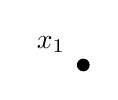
\begin{tikzpicture} 
            \node[draw,circle,fill=black,scale=0.2,label={[label distance=1pt]165:$x_1$}] at (0,0) (x1) {$x_1$}; 
          \end{tikzpicture} & point \\
    \hline
    $1$ & 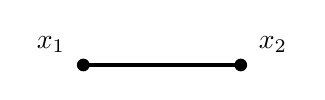
\begin{tikzpicture} 
            \node[draw,circle,fill=black,scale=0.2,label={[label distance=1pt]165:$x_1$}] at (-1,0) (x1) {$x_1$}; 
            \node[draw,circle,fill=black,scale=0.2,label={[label distance=1pt]15:$x_2$}] at (1,0) (x2) {$x_2$}; 
            \draw[very thick] (x1) -- (x2); 
          \end{tikzpicture} & edge \\
    \hline
    $2$ & 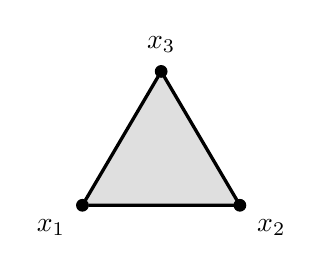
\begin{tikzpicture}
            \fill[gray!25] (-1,0) -- (1,0) -- (0,1.7) -- cycle;
            \node[draw,circle,fill=black,scale=0.2,label={[label distance=1pt]210:$x_1$}] at (-1,0) (x1) {$x_1$};
            \node[draw,circle,fill=black,scale=0.2,label={[label distance=1pt]-30:$x_2$}] at (1,0) (x3) {$x_2$};
            \node[draw,circle,fill=black,scale=0.2,label={[label distance=1pt]90:$x_3$}] at (0,1.7) (x2) {$x_3$};
            \draw[very thick] (x1) -- (x2) -- (x3) -- (x1);
          \end{tikzpicture} & triangle \\
    \hline
    $3$ & 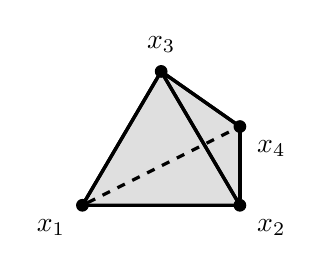
\begin{tikzpicture} 
            \fill[gray!25] (-1,0) -- (1,0) -- (1,1) -- (0,1.7);
            \node[draw,circle,fill=black,scale=0.2,label={[label distance=1pt]210:$x_1$}] at (-1,0) (x1) {$x_1$};
            \node[draw,circle,fill=black,scale=0.2,label={[label distance=1pt]-30:$x_2$}] at (1,0) (x2) {$x_2$};
            \node[draw,circle,fill=black,scale=0.2,label={[label distance=1pt]90:$x_3$}] at (0,1.7) (x3) {$x_3$};
            \node[draw,circle,fill=black,scale=0.2,label={[label distance=1pt]-30:$x_4$}] at (1,1) (x4) {$x_4$};
            \draw[very thick] (x1) -- (x2) -- (x3) -- (x1);
            \draw[very thick] (x1) -- (x2) -- (x4);
            \draw[very thick] (x1) -- (x3) -- (x4);
            \draw[very thick,dashed] (x1) -- (x4);
            \draw[very thick] (x2) -- (x3) -- (x4) -- (x2);
          \end{tikzpicture} & tetrahedron \\
    \hline
\end{tabular}
}
\end{center}

\begin{definition}
    A \emph{simplicial complex} $\Delta$ on a vertex set $V$ is a set of subsets of $V$ which is closed under taking subsets.
    The \emph{dimension} of $\Delta$ is the maximum dimension of a face of $\Delta$.
\end{definition}

While the definition of a simplicial complex might seem a bit abstract, this is really just making sure that if, for instance, I have a filled in triangle, then I better have the triangle's edges and vertices as well.
With this definition, however, we now have a lot of combinatorics at our disposal as simplicial complexes have much expressive power in modeling mathematical objects.

\begin{remark}
    It will not really pop up for this project, but simplicial complexes connect enumerative combinatorics (simplicial complexes), algebra (Stanley-Reisner theory), and topology (manifolds).
    In a rough sense, since a simplex models $\RR^d$, simplicial complexes give us a way to construct and model topological spaces by gluing simplices together to model more complicated topological spaces (see \emph{triangulations} in algebraic topology).
\end{remark}

\begin{definition}
    The $f$-vector of a $d$-dimensional simplicial complex $\Delta$ is the vector $(f_{-1}, f_0, f_1, \dots, f_d)$ where $f_{-1} = 1$ and $f_i$ records the number of $i$-dimensional faces of $\Delta$.
\end{definition}

\begin{exercise}
    Compute the $f$-vector of a $d$-dimensional simplex.
    Compute the $f$-vector of a \emph{hollow} $d$-dimensional simplex; this is the $f$-vector of the \emph{boundary} of the simplex.
    How do the $f$-vectors differ?
\end{exercise}

\begin{example}
    Consider the simplicial complex $\Delta$ below, where all the black components comprise $\Delta$ and the red and blue dashed lines are excluded. 
    \begin{center}
    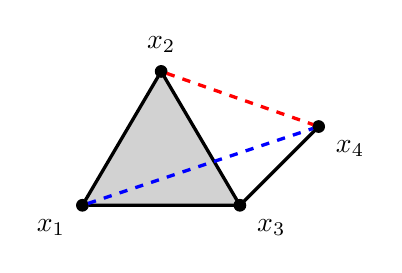
\begin{tikzpicture}
        \fill[gray!35] (-3,0) -- (-2,1.7) -- (-1,0) -- (-3,0);
        \node[draw,circle,fill=black,scale=0.2,label={[label distance=1pt]210:$x_1$}] at (-3,0) (A) {$x_1$};
        \node[draw,circle,fill=black,scale=0.2,label={[label distance=1pt]90:$x_2$}] at (-2,1.7) (B) {$x_2$};
        \node[draw,circle,fill=black,scale=0.2,label={[label distance=1pt]-30:$x_3$}] at (-1,0) (C) {$x_3$};
        \node[draw,circle,fill=black,scale=0.2,label={[label distance=1pt]-30:$x_4$}] at (0,1) (D) {$x_4$};
        \draw[very thick] (A) -- (B) -- (C) -- (A);
        \draw[very thick] (C) -- (D);
        \draw[very thick, color=blue, dashed] (A) -- (D);
        \draw[very thick, color=red, dashed] (B) -- (D);
    \end{tikzpicture}
    \end{center}
    So, then (only keeping track of indices) we have
    \begin{align*}
        \Delta &= \left\{ \{ 1,2,3 \}, \{ 1,2 \}, \{ 1,3 \}, \{ 2,3 \}, \{ 3,4 \}, \{ 1 \}, \{ 2 \}, \{ 3 \}, \{ 4 \}, \emptyset \right\} \\
        &= \langle \{ 1,2,3 \}, \{ 3,4 \} \rangle \\
        &= \langle 123, 34 \rangle.
    \end{align*}
    Note that $\Delta$ is not a \emph{simplex}; it is a \emph{simplicial complex}.
    It is $2$-dimensional (the filled-in triangle has dimension $2$), and its $f$-vector is $(1, 4, 4, 1)$.
\end{example}

\vspace*{1cm}

\noindent {\bf See Also}: Section 5.1 of~\cite{schenck_computational_2003}.

\vspace*{1cm}


\subsection{The Stanley-Reisner Correspondence}
Since a simplicial complex is closed under subsets, it can be succinctly described by its top-dimensional faces.
The key insight by Stanley and Reisner is that it can equivalently be described via its minimal non-faces.

\begin{exercise}
    Prove that if $\{ i_1, \dots, i_s \}$ is not a face of $\Delta$, then no superset of $\{ i_1, \dots, i_s \}$ is a face of $\Delta$.
\end{exercise}

\begin{definition}
    Let $\Delta$ be a simplicial complex on $n$ vertices.
    The \emph{Stanley-Reisner ideal} of $\Delta$ is the ideal $I_\Delta \subseteq \KK[x_1,\dots,x_n]$ generated by the non-faces of $\Delta$; i.e.,
    \begin{equation*}
        I_\Delta \coloneqq \langle x_{i_1} \dots x_{i_s} \, \colon \, \{ i_1, \dots, i_s \} \text{ is not a face of } \Delta \rangle.
    \end{equation*}
    The \emph{Stanley-Reisner ring} of $\Delta$ is the quotient $\KK[\Delta] \coloneqq R/I_\Delta$; this is sometimes also called the \emph{face ring} of $\Delta$.
\end{definition}

\begin{theorem}
    There is a one-to-one correspondence between simplicial complexes on $n$ vertices and squarefree, monomial ideals in $\KK[x_1,\dots,x_n]$.
\end{theorem}

\begin{example}
    Consider the simplicial complex $\Delta$ from before:
    \begin{center}
    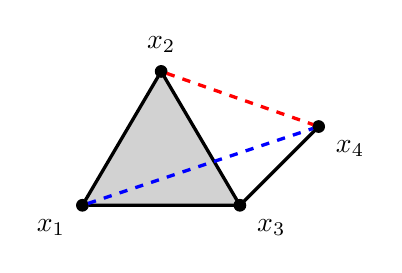
\begin{tikzpicture}
        \fill[gray!35] (-3,0) -- (-2,1.7) -- (-1,0) -- (-3,0);
        \node[draw,circle,fill=black,scale=0.2,label={[label distance=1pt]210:$x_1$}] at (-3,0) (A) {$x_1$};
        \node[draw,circle,fill=black,scale=0.2,label={[label distance=1pt]90:$x_2$}] at (-2,1.7) (B) {$x_2$};
        \node[draw,circle,fill=black,scale=0.2,label={[label distance=1pt]-30:$x_3$}] at (-1,0) (C) {$x_3$};
        \node[draw,circle,fill=black,scale=0.2,label={[label distance=1pt]-30:$x_4$}] at (0,1) (D) {$x_4$};
        \draw[very thick] (A) -- (B) -- (C) -- (A);
        \draw[very thick] (C) -- (D);
        \draw[very thick, color=blue, dashed] (A) -- (D);
        \draw[very thick, color=red, dashed] (B) -- (D);
    \end{tikzpicture}
    \end{center}
    Its Stanley-Reisner ideal is $(x_1 x_4, x_2 x_4) \subseteq \KK[x_1,x_2,x_3,x_4]$.
\end{example}

Intuitively, the Stanley-Reisner correspondence is using the ideal to set relations where if a simplicial complex does \emph{not} have a face, then the corresponding monomial should be set to $0$.
But now, any problem about simplicial complexes can be translated to commutative algebra where high-tech machinery can be applied, or vice versa where complicated algebraic objects can become more substantive and hands-on with combinatorics.
However, while you should learn to love Stanley-Reisner theory, care must be taken not to get too optimistic all of the time: simplicial complexes can be used to model most topological spaces, so studying \emph{all} simplicial complexes will be hard in general.

\begin{exercise}
    \label{exercise:hollow octahedron}
    Consider the hollow octahedron, i.e., the boundary of the octahedron (all of the triangular faces are included):
    \begin{center}
    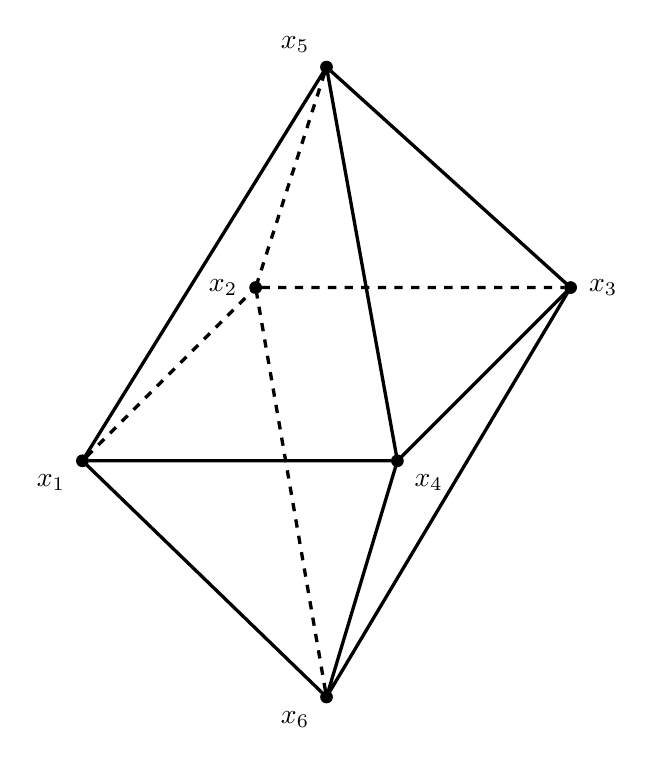
\begin{tikzpicture}
        \node[draw,circle,fill=black,scale=0.2,label={[label distance=1pt]210:$x_1$}] at (0,0) (x1) {$x_1$};
        \node[draw,circle,fill=black,scale=0.2,label={[label distance=1pt]180:$x_2$}] at (2.2,2.2) (x2) {$x_2$};
        \node[draw,circle,fill=black,scale=0.2,label={[label distance=1pt]0:$x_3$}] at (6.2,2.2) (x3) {$x_3$};
        \node[draw,circle,fill=black,scale=0.2,label={[label distance=1pt]-30:$x_4$}] at (4,0) (x4) {$x_4$};
        \node[draw,circle,fill=black,scale=0.2,label={[label distance=1pt]150:$x_5$}] at (3.1,5) (x5) {$x_5$};
        \node[draw,circle,fill=black,scale=0.2,label={[label distance=1pt]210:$x_6$}] at (3.1,-3) (x6) {$x_6$};
        \draw[very thick, dashed] (x1) -- (x2) -- (x3);
        \draw[very thick] (x3) -- (x4) -- (x1);
        \draw[very thick] (x1) -- (x5);
        \draw[very thick, dashed] (x5) -- (x2);
        \draw[very thick] (x3) -- (x5) -- (x4);
        \draw[very thick] (x1) -- (x6);
        \draw[very thick, dashed] (x6) -- (x2);
        \draw[very thick] (x3) -- (x6) -- (x4);
    \end{tikzpicture}
    \end{center}
    Compute its Stanley-Reisner ideal. What is the $f$-vector of the hollow octahedron?
\end{exercise}

It turns out there is another vector---which is equivalent to the $f$-vector---that has better combinatorial properties.

\begin{definition}
    The \emph{$h$-vector} of a $(d-1)$-dimensional simplicial complex is given by
    \begin{equation*}
        h_j = \sum_{i=0}^j (-1)^{j-i} \binom{d-i}{j-i} f_{i-1}.
    \end{equation*}
    Moreover,
    \begin{equation*}
        f_j = \sum_{i=0}^{j+1} \binom{d-i}{i+j-1} h_i.
    \end{equation*}
\end{definition}

\begin{proposition}
    Suppose $\Delta$ is a $(d-1)$-dimensional simplicial complex.
    Then its $h$-vector $(h_0,h_1,\dots,h_d)$ can be computed from its $f$-vector via the following recurrence relations:
    \begin{equation*}
        \begin{cases}
            h_0^i = 1 & -1 \leq i \leq d \\
            h_{i+1}^i = f_i & -1 \leq i \leq d-1 \\
            h_k^i = h_k^{i-1} - h_{k-1}^{i-1} & 1 \leq k \leq i \leq d
        \end{cases}
    \end{equation*}
    and by setting $h_k = h_k^d$ for $0 \leq k \leq d$.
\end{proposition}

\begin{example}
    Consider the square cone $\Delta$ (the triangular faces are included, but the top square face is not):
    \begin{center}
    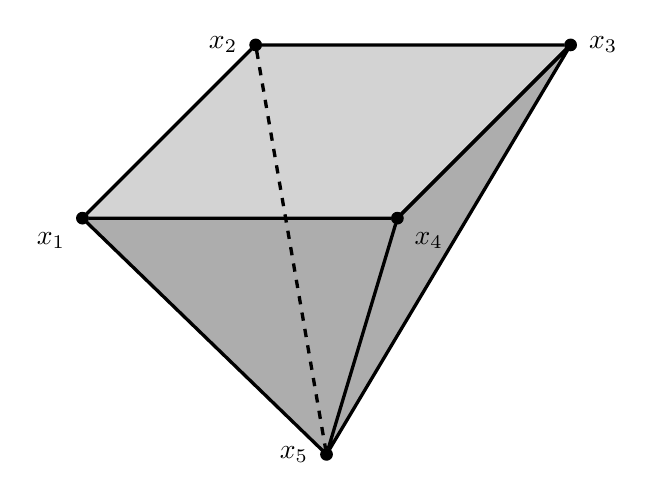
\begin{tikzpicture}
        \fill[gray,opacity=0.35] (0,0) -- (2.2,2.2) -- (3.1,-3) -- cycle;
        \fill[gray,opacity=0.35] (2.2,2.2) -- (6.2,2.2) -- (3.1,-3) -- cycle;
        \fill[gray,opacity=0.45] (6.2,2.2) -- (4,0) -- (3.1,-3) -- cycle;
        \fill[gray,opacity=0.45] (0,0) -- (4,0) -- (3.1,-3) -- cycle;
        \node[draw,circle,fill=black,scale=0.2,label={[label distance=1pt]210:$x_1$}] at (0,0) (x1) {$x_1$};
        \node[draw,circle,fill=black,scale=0.2,label={[label distance=1pt]180:$x_2$}] at (2.2,2.2) (x2) {$x_2$};
        \node[draw,circle,fill=black,scale=0.2,label={[label distance=1pt]0:$x_3$}] at (6.2,2.2) (x3) {$x_3$};
        \node[draw,circle,fill=black,scale=0.2,label={[label distance=1pt]-30:$x_4$}] at (4,0) (x4) {$x_4$};
        \node[draw,circle,fill=black,scale=0.2,label={[label distance=1pt]180:$x_5$}] at (3.1,-3) (x5) {$x_5$};
        \draw[very thick] (x1) -- (x2) -- (x3) -- (x4) -- (x1);
        \draw[very thick] (x1) -- (x5);
        \draw[very thick, dashed] (x2) -- (x5);
        \draw[very thick] (x3) -- (x4) -- (x5) -- (x3);
    \end{tikzpicture}
    \end{center}
    We can see that the $f$-vector of $\Delta$ is $(1,5,8,4)$.
    The recurrence relations for the $h$-vector are actually describing a Pascal triangle-like recurrence.
    To get the $h$-vector of $\Delta$, construct a triangle with $1$'s along the left diagonal and the $f$-vector along the right diagonal:
    \begin{center}
    \begin{tikzcd}
         &  &  &  & 1 &  &  &  &  \\
         &  &  & 1 &  & f_0 &  &  &  \\
         &  & 1 &  &  &  & f_1 &  &  \\
         & 1 &  &  &  &  &  & f_2 &  \\
        1 &  &  &  &  &  &  &  & 0
    \end{tikzcd}
    \end{center}
    Then follow Pascal's identity to fill out the rest of the triangle: subtract the upper-left neighbor from the upper-right neighbor.
    \begin{center}
    \begin{tikzcd}
         &  &  &  & 1 &  &  &  &  \\
         &  &  & 1 \arrow[dr] &  & 5 \arrow[dl] &  &  &  \\
         &  & 1 \arrow[dr] &  & 4 \arrow[dr] \arrow[dl] &  & 8 \arrow[dl] &  &  \\
         & 1 \arrow[dr] &  & 3 \arrow[dr] \arrow[dl] &  & 4 \arrow[dr] \arrow[dl] &  & 4 \arrow[dl] &  \\
        1 &  & 2 &  & 1 &  & 0 &  & 0
    \end{tikzcd}
    \end{center}
    Lo and behold, the bottom row $(1,2,1)$ is the $h$-vector of $\Delta$!
\end{example}

\begin{exercise}
    Compute the $h$-vector of the boundary of the hollow octahedron (the simplicial complex from \Cref{exercise:hollow octahedron}).
\end{exercise}

\vspace*{1cm}

\noindent {\bf See Also}: Section 5.2 of~\cite{schenck_computational_2003}.

\vspace*{1cm}


\subsection{Combinatorial Commutative Algebra}
To really illustrate some of the utility of the $h$-vector, the following are some results which let you recover the number of top-dimensional faces of $\Delta$, as well as the numerator of its Hilbert-Poincar\'e series.

\begin{proposition}
    Suppose $\Delta$ is the boundary of a $d$-dimensional convex polytope.
    Then $f_{d-1} = h_0 + \dots + h_d$.
\end{proposition}

\begin{theorem}
    \label{theorem:sr hilbert poincare}
    Suppose $\Delta$ is the boundary of a $d$-dimensional convex polytope, and let $\KK[\Delta]$ be its Stanley-Reisner ring.
    Then the Hilbert-Poincar\'e series of $\KK[\Delta]$ can be expressed as
    \begin{equation*}
        P_{\KK[\Delta]}(t) = \sum_{i=0}^d \frac{f_{i-1} t^i}{(1-t)^i} = \frac{h_0 + h_1 t + \dots + h_d t^d}{(1-t)^d}.
    \end{equation*}
\end{theorem}

\begin{example}
    Let $\Delta$ be the hollow octahedron from \Cref{exercise:hollow octahedron}.
    If you did not skip ahead, you should have found that its Stanley-Reisner ideal is $(x_1 x_3, x_2 x_4, x_5 x_6) \subseteq \KK[x_1,\dots,x_6]$, its $f$-vector is $(1,6,12,8)$, and its $h$-vector is $(1,3,3,1)$.
    Computing the free resolution of $\KK[\Delta]$, we get
    \begin{equation*}
        0 \leftarrow R/I_\Delta \leftarrow R \xleftarrow[]{} R(-2)^3 \xleftarrow[]{} R(-4)^3 \xleftarrow[]{} R(-6) \leftarrow 0.
    \end{equation*}
    If we rewrite the shifts in the resolution in a way more amenable to the Betti table convention, we then get
    \begin{equation*}
        0 \leftarrow R/I_\Delta \leftarrow R \xleftarrow[]{} R(-(1+1))^3 \xleftarrow[]{} R(-(2+2))^3 \xleftarrow[]{} R(-(3+3)) \leftarrow 0,
    \end{equation*}
    and so the Betti table of $\KK[\Delta]$ is
    \begin{equation*}
        \Betti(\KK[\Delta]) =
        \begin{array}{r|cccc}
          & 0 & 1 & 2 & 3 \\
        \hline
        \text{total} & 1 & 3 & 3 & 1 \\
        \hline
         0 & 1 & . & . & . \\
         1 & . & 3 & . & . \\
         2 & . & . & 3 & . \\
         3 & . & . & . & 1
    \end{array}.
    \end{equation*}
    However, in particular, notice that the ranks of the $R(\text{--})$ appearing in the free resolution of $\KK[\Delta]$ are exactly the entries of the $h$-vector!
    If you are feeling ambitious, try computing the Hilbert series of $\KK[\Delta]$ by hand.
    
    It has a denominator of $(1-t)^6$, but we can simplify it a bit to get down to a denominator of $(1-t)^3$.
    You should get
    \begin{equation*}
        \HS(\KK[\Delta]) = \frac{1 - 3t^2 + 3t^4 - t^6}{(1-t)^6} = \frac{1 + 3t + 3t^2 + t^3}{(1-t)^3}.
    \end{equation*}
    This is \Cref{theorem:sr hilbert poincare} in action!
\end{example}

\vspace*{1cm}

\noindent {\bf See Also}: Section 5.2 of~\cite{schenck_computational_2003}.

\vspace*{1cm}


\subsection{Macaulay2 Code}
\begin{verbatim}
-- Exercise 4.5 (f-vectors of simplices)
needsPackage "SimplicialComplexes"
netList for d from -1 to 5 list (
    R = QQ[x_0..x_d];
    delta = simplexComplex(d, R);
    fVector delta
)

netList for d from 1 to 5 list (
    R = QQ[x_0..x_d];
    dSubsets = subsets(R_*, d);
    delta = simplicialComplex apply(dSubsets, S -> product S);
    fVector delta
)


-- Example 4.6 (triangle + edge)
restart
needsPackage "SimplicialComplexes"
R = QQ[x_1..x_4]
delta = simplicialComplex {x_1*x_2*x_3, x_3*x_4}
faces delta
fVector delta


-- Example 4.10 (Stanley-Reisner ideal of triangle + edge)
ideal delta


-- Exercise 4.11 (hollow octahedron)
restart
needsPackage "SimplicialComplexes"
R = QQ[x_1..x_6]
delta = simplicialComplex {x_1*x_2*x_5, x_2*x_3*x_5, x_3*x_4*x_5, x_1*x_4*x_5,
                           x_1*x_2*x_6, x_2*x_3*x_6, x_3*x_4*x_6, x_1*x_4*x_6}
I = ideal delta
fVector delta


-- Example 4.18 (resolution of hollow octahedron)
res I
betti res I 
hilbertSeries I
hilbertSeries(I, Reduce=>true)
\end{verbatim}






\newpage
\section{Putting It All Together}
\textit{Which simplicial complexes have Lefschetz properties?}

\vspace*{2.5cm}

To every simplicial complex, we can get its Stanley-Reisner ideal.
We can then throw in powers of the variables to get an Artinian algebra.
With this process, we can then ask for which simplicial complexes do we get an Artinian algebra with Lefschetz properties?

\vspace*{2.5cm}

\begin{tldr}
    \phantom{ }
    \begin{itemize}
        \item We can obtain Artinian algebras from simplicial complexes.
        
        \item We have to be careful about which powers of variables to throw in to the ideal to get an Artinian algebra.

        \item Hopefully the combinatorics of the simplicial complex let us say something about the Betti numbers, and subsequently about Lefschetz properties.
    \end{itemize}
\end{tldr}


\newpage
We will start with a simplicial complex, but need to get something Artinian in order to think about Lefschetz properties.
Let $R = \KK[x_1,\dots,x_n]$ and $I = I_\Delta$ the Stanley-Reisner ideal of a simplicial complex $\Delta$. 
Set $A \coloneqq R/(I+J)$, where $J = (x_i^2 \, \colon \, 1 \leq i \leq n)$.

\begin{exercise}
    Show that $A$ is Artinian.
\end{exercise}


\subsection{The Project}
We will call $A$ the \emph{standard Artinian reduction} of $I_\Delta$: we took $I_\Delta$ and threw in powers of the variables as generators to produce an Artinian algebra.
Since $A$ is Artinian, we can now ask all the Lefschetz-related questions.
In particular:

\begin{question}
    \label{question:simplicial complexes lefschetz}
    Which simplicial complexes $\Delta$ has the weak (strong) Lefschetz property?
\end{question}

This is probably a bit too hard of a question, but we can use a result from~\cite{grate_betti_2024}.
In a nutshell, by looking at the Betti table of an Artinian algebra $A$, if it has a certain pattern in its ``top'' row, then we might be able to say something.

\begin{definition}{\cite[Definition~1]{grate_betti_2024}}
    A Betti table $B$ has an $(n,d)$-Koszul tail if it has an upper left principal block of the form
    \begin{equation*}
        \begin{array}{r|ccccccccc}
              & 0 & 1 & 2 & 3 & \dots & n-2 & n-1 & n & n+1 \\
            \hline
            0 & 1 & . & . & . & \dots & . & . & . & * \\
            1 & . & . & . & . & \dots & . & . & . & * \\
            \vdots & \vdots & \vdots & \vdots & \vdots & \ddots & \vdots & \vdots & \vdots & * \\
            d-1 & . & . & . & . & \dots & . & . & . & * \\
            d & . & n & \binom{n}{2} & \binom{n}{3} & \dots & \binom{n}{n-2} & n & 1 & * \\
            d+1 & * & * & * & * & * & * & * & * & *
        \end{array}.
    \end{equation*}
    If $B$ has an $(n,d)$-Koszul tail and is the Betti table for an Artinian ring $\KK[x_1,\dots,x_n]/I$---i.e., all of the entries in the columns \emph{after} the tail are zero---then we say $B$ has a \emph{maximal} $(n,d)$-Koszul tail.
\end{definition}

\begin{theorem}{\cite[Theorem~2]{grate_betti_2024}}\label{theorem:grate-schenck}
    Suppose $A = R/I$ is an Artinian algebra.
    If the Betti table of $A$ has a maximal $(n,d)$-Koszul tail, then $A$ does not have the WLP.
\end{theorem}

Using \Cref{theorem:grate-schenck} and trying to work combinatorially, we just need to associate an Artinian algebra to a simplicial complex.
This gives an avenue of attack for \Cref{question:simplicial complexes lefschetz}:

\begin{question}\label{question:simplicial complexes koszul tails}
    Which simplicial complexes $\Delta$ have Stanley-Reisner ideals $I_\Delta$ whose standard Artinian reduction have maximal Koszul tails?
    In other words, if $A = R / (I_\Delta + J)$, then when does $\Betti(A)$ have a maximal Koszul tail?
\end{question}

The dream is to not only find examples of simplicial complexes affirmatively answer \Cref{question:simplicial complexes koszul tails}, but to characterize them.
If this is possible, this would mean that there is a \emph{combinatorial interpretation} of Koszul tails in the Stanley-Reisner regime.

However, working with the \emph{standard} Artinian reduction of $I_\Delta$ might be too restrictive to apply \Cref{theorem:grate-schenck}.
To remedy this, we can consider more general Artinian reductions of $I_\Delta$:
\begin{itemize}
    \item The \emph{degree $d$ Artinian reduction} of $I_\Delta$ is the Artinian algebra $A = R / (I_\Delta + J)$, where
    \begin{equation*}
        J = (x_i^d \, \colon \, 1 \leq i \leq n).
    \end{equation*}
    Note that when $d=2$, this is the standard Artinian reduction of $I_\Delta$ from before.

    \item The \emph{$(d_1,\dots,d_n)$-Artinian reduction} of $I_\Delta$ is the Artinian algebra $A = R / (I_\Delta + J)$, where
    \begin{equation*}
        J = (x_i^{d_i} \, \colon \, 1 \leq i \leq n).
    \end{equation*}
    When $d_i=2$ for all $i$, this is the standard Artinian reduction of $I_\Delta$ from before, and when all the $d_i$ are equal, this is the degree $d$ Artinian reduction of $I_\Delta$ from before, too.
\end{itemize}

\begin{question}
    Fix a simplicial complex $\Delta$.
    Which Artinian reductions of $I_\Delta$ have (maximal) Koszul tails?
    What kind of region (e.g., convex) do these form in $\NN^d$?
\end{question}


\subsection{Literature for WLP of Monomial Ideals}
Given a Stanley-Reisner ring $R/I_\Delta$, we can throw in the squares of the variables to get an Artinian algebra; more precisely, if $P = (x_1^2,\dots,x_n^2)$, then we can consider $A = R/(I_\Delta + P)$.
Plenty of results are known about these algebras, so the following sections summarize a few of these.

\subsubsection{\href{https://arxiv.org/abs/1706.05058}{Migliore-Nagel-Schenck}}
\begin{lemma}{\cite[Lemma 2.1]{migliore_quadratic_2020}}
    If $A = R/(I_\delta + P)$, then the Hilbert series of $A$ is
    \begin{equation*}
        \HS(A) = \sum f_{i-1} t^i.
    \end{equation*}
\end{lemma}

\begin{corollary}{\cite[Corollary 2.2]{migliore_quadratic_2020}}
    The algebra $A = R/(I_\Delta + P)$ is level if and only if the flag complex is pure.
\end{corollary}

\begin{definition}
    Suppose $\Delta$ is a simplicial complex and $\partial \Delta$ is its boundary.
    For a face $\sigma \in \Delta$, the \emph{star} of $\sigma$ is
    \begin{equation*}
        \sstar(\sigma) = \{ \tau \in \Delta \, \colon \, \sigma \subseteq \tau \},
    \end{equation*}    
    and the \emph{link} of $\sigma$ is
    \begin{equation*}
        \link(\sigma) = \partial(\sstar(\sigma)).
    \end{equation*}
\end{definition}

\begin{lemma}{\cite[Lemma 2.3]{migliore_quadratic_2020}}
    SOME LEMMA ABOUT REMOVING A VERTEX.
\end{lemma}

\begin{lemma}{\cite[Lemma 2.4]{migliore_quadratic_2020}}
    SOME LEMMA ABOUT REMOVING AN EDGE.
\end{lemma}


\subsubsection{\href{https://www.sciencedirect.com/science/article/pii/S000187080700299X}{Mermin-Peeva-Stillman}}
\begin{theorem}{\cite[Theorem 2.1(4)]{mermin_ideals_2008}}
    Let $I \subseteq R = \KK[x_1,\dots,x_n]$ be a squarefree monomial ideal.
    Then the graded Betti numbers of $R / (I_\Delta + P)$ are
    \begin{equation*}
        \beta_{p,s}\left( R / (I_\Delta + P) \right) = \sum_{i=0}^n \left( \sum_{\abs{\sigma} = i} \beta_{p-i, s-2i} \left( R / (I \colon \sigma) \right) \right).
    \end{equation*}
\end{theorem}


\subsubsection{\href{https://arxiv.org/abs/2112.09434}{Dao-Nair}}
\begin{proposition}{\cite[Proposition 2.2]{dao_lefschetz_2024}}
    Set $A(\Delta) = R / (I_\Delta + P)$.
    \begin{enumerate}[label=(\roman*)]
        \item The monomials in $R/(I_\Delta + P)$ are in bijection with the faces of $\Delta$.
        For $i > 0$, $A(\Delta)_i$ is a $\KK$-vector space with a basis given by $\{ x_F \, \colon \, F \text{ is an } (i-1)\text{-face of } \Delta \}$.

        \item $\displaystyle \HS(A(\Delta)) = \sum_{i \geq 0} f_{i-1}(\Delta) t^i$.

        \item $\displaystyle A(\Delta_i) = \bigoplus_{j \leq i+1} (A(\Delta))_j$.

        \item A top socle of $A(\Delta)$ is given by $x_F$, where $F$ is any facet of $\Delta$ of dimension $\dim(\Delta)$.
        The top socle degree is $\dim(\Delta) + 1$, and this number is the Castelnuovo-Mumford regularity of $A(\Delta)$.
    \end{enumerate}
\end{proposition}

\begin{proposition}{\cite[Proposition 2.6]{dao_lefschetz_2024}}
    Given a simplicial complex $\Delta$ of dimension $d$, if $\dim_{\KK}{A(\Delta)_i} > \dim_{\KK}(A(\Delta)_{i+1})$ for some $i \geq 1$ and if WLP holds in degree $i$, then WLP holds in all degrees greater than $i$.
\end{proposition}

\begin{theorem}{\cite[Theorem 3.3]{dao_lefschetz_2024}}
    \begin{enumerate}[label=(\roman*)]
        \item If $\dim_{\KK}{A(\Delta)_2} \geq \dim_{\KK}{A(\Delta)_1}$, then WLP holds in degree $1$ if and only if the $1$-skeleton of $\Delta$ has no bipartite components.

        \item If $\dim_{\KK}{A(\Delta)_2} < \dim_{\KK}{A(\Delta)_1}$, then WLP holds in degree $1$ if and only if each bipartite component of the $1$-skeleton of $\Delta$ (if it exists) is a tree and each non-bipartite component satisfies the property that the number of edges in the component is equal to the number of vertices in the component.
        Furthermore, WLP holds in degree $1$ implies WLP holds in all degrees.
    \end{enumerate}
\end{theorem}

\begin{corollary}{\cite[Corollary 3.6]{dao_lefschetz_2024}}
    Suppose $A(\Delta)$ has WLP in degree $1$.
    If $\dim_{\KK}{A(\Delta)_2} \leq \dim_{\KK}{A(\Delta)_1}$, then $\reg(A(\Delta)) \leq 3$.
\end{corollary}

\begin{remark}
    \cite{dao_lefschetz_2024} contains more general results about WLP with respect to pseudo-manifolds...
\end{remark}

\subsubsection{\href{https://arxiv.org/abs/2306.13274}{Holleben}}
\begin{definition}{\cite[Definition 17]{holleben_lefschetz_2024}}
    Let $\Delta$ be a simplicial complex and $F_i$ the set of all $i$-dimensional faces of $\Delta$.
    The matrix $M(\Delta, i)$ is the $f_i \times f_{i-1}$ matrix such that the rows are labeled by $i$-faces, the columns are labeled by $(i-1)$-faces, and
    \begin{equation*}
        M(\Delta, i)_{j,k} = \begin{cases}
            1 & \text{if the } j \text{-th element of } F_i \text{ contains the } k \text{-th element of } F_{i-1} \\
            0 & \text{otherwise}
        \end{cases}.
    \end{equation*}
    This matrix is called the \emph{$i$-th incidence matrix} of $\Delta$.
\end{definition}

\begin{lemma}{\cite[Lemma 23]{holleben_lefschetz_2024}}
    Let $\Delta$ be a simplicial complex, $A = A(\Delta)$, and $L = x_1 + \dots x_n$.
    The matrix that represents the multiplication map $\cdot L \colon A_i \to A_{i+1}$ is $M(\Delta, i)$, where the entries of $M(\Delta,i)$ are taken to be in $\KK$, the base field of $A$.
\end{lemma}

\begin{theorem}{\cite[Theorem 54]{holleben_lefschetz_2024}}
    Let $\Delta$ be a simplicial complex such that $f_0 \leq f_1$.
    Then one of the two following statements holds:
    \begin{enumerate}[label=(\arabic*)]
        \item $A(\Delta)$ fails the WLP in degree $1$ in every characteristic.

        \item $A(\Delta)$ has the WLP in degree $1$ in every characteristic except characteristic $2$.
    \end{enumerate}
\end{theorem}

\begin{definition}{\cite[Definition 55]{holleben_lefschetz_2024}}
    Let $I \subseteq R = \KK[x_1,\dots,x_n]$ be a monomial ideal such that $A = R/I$ is Artinian.
    The \emph{underlying graph} of $A$, denoted $G_A$, has vertex set $\{ x_i \, \colon \, x_i \not\in I \}$ and has edge $\{ x_i, x_k \}$ (possibly with $i=j$) if and only if $x_i x_j \not\in I$.
\end{definition}

\begin{theorem}{\cite[Theorem 58]{holleben_lefschetz_2024}}
    Let $R = \KK[x_1,\dots,x_n]$ and $I$ a monomial ideal.
    Assume $A = R/I$ is Artinian and $\dim_{\KK}{A_1} \leq \dim_{\KK}{A_2}$.
    Then either $A$ has the WLP in degree $1$ in every characteristic $\neq 2$, or $A$ fails the WLP in degree $1$ in every characteristic $\neq 2$.

    Moreover, $A$ has the WLP in characteristic zero if and only if every connected component of the \emph{underlying graph} of $A$ contains a subgraph that is either
    \begin{enumerate}[label=(\arabic*)]
        \item a tree with one loop, or
        
        \item a graph that has only one cycle of odd length.
    \end{enumerate}
\end{theorem}

\begin{question}{\cite[Question 61]{holleben_lefschetz_2024}}
    What are necessary and sufficient conditions for a squarefree monomial ideal to be the \emph{incidence ideal} of some simplicial complex?
\end{question}


\subsection{Macaulay2 Code}
The majority of code will hosted via GitHub in Sean's \href{https://github.com/seangrate/Koszul-SR-Complexes/blob/main/koszul_tails.m2}{\tt Koszul-SR-Complexes} repository.


\newpage
\bibliographystyle{amsplain}
\bibliography{./refs}

\end{document}